\documentclass[10pt]{beamer}

\usepackage{FiraSans}
\usepackage[T1]{fontenc}
\usepackage[utf8]{inputenc}
\usetheme{metropolis}

\usetikzlibrary{calc}
\usepackage{xcolor}
\usetikzlibrary{overlay-beamer-styles}

\title{How JPEG works}
\date{February 9, 2021}
\author{Krzysztof Antoniak}

\begin{document}
\maketitle

\section{Section}

\begin{frame}[c,plain]
	\begin{figure}
		\centering
		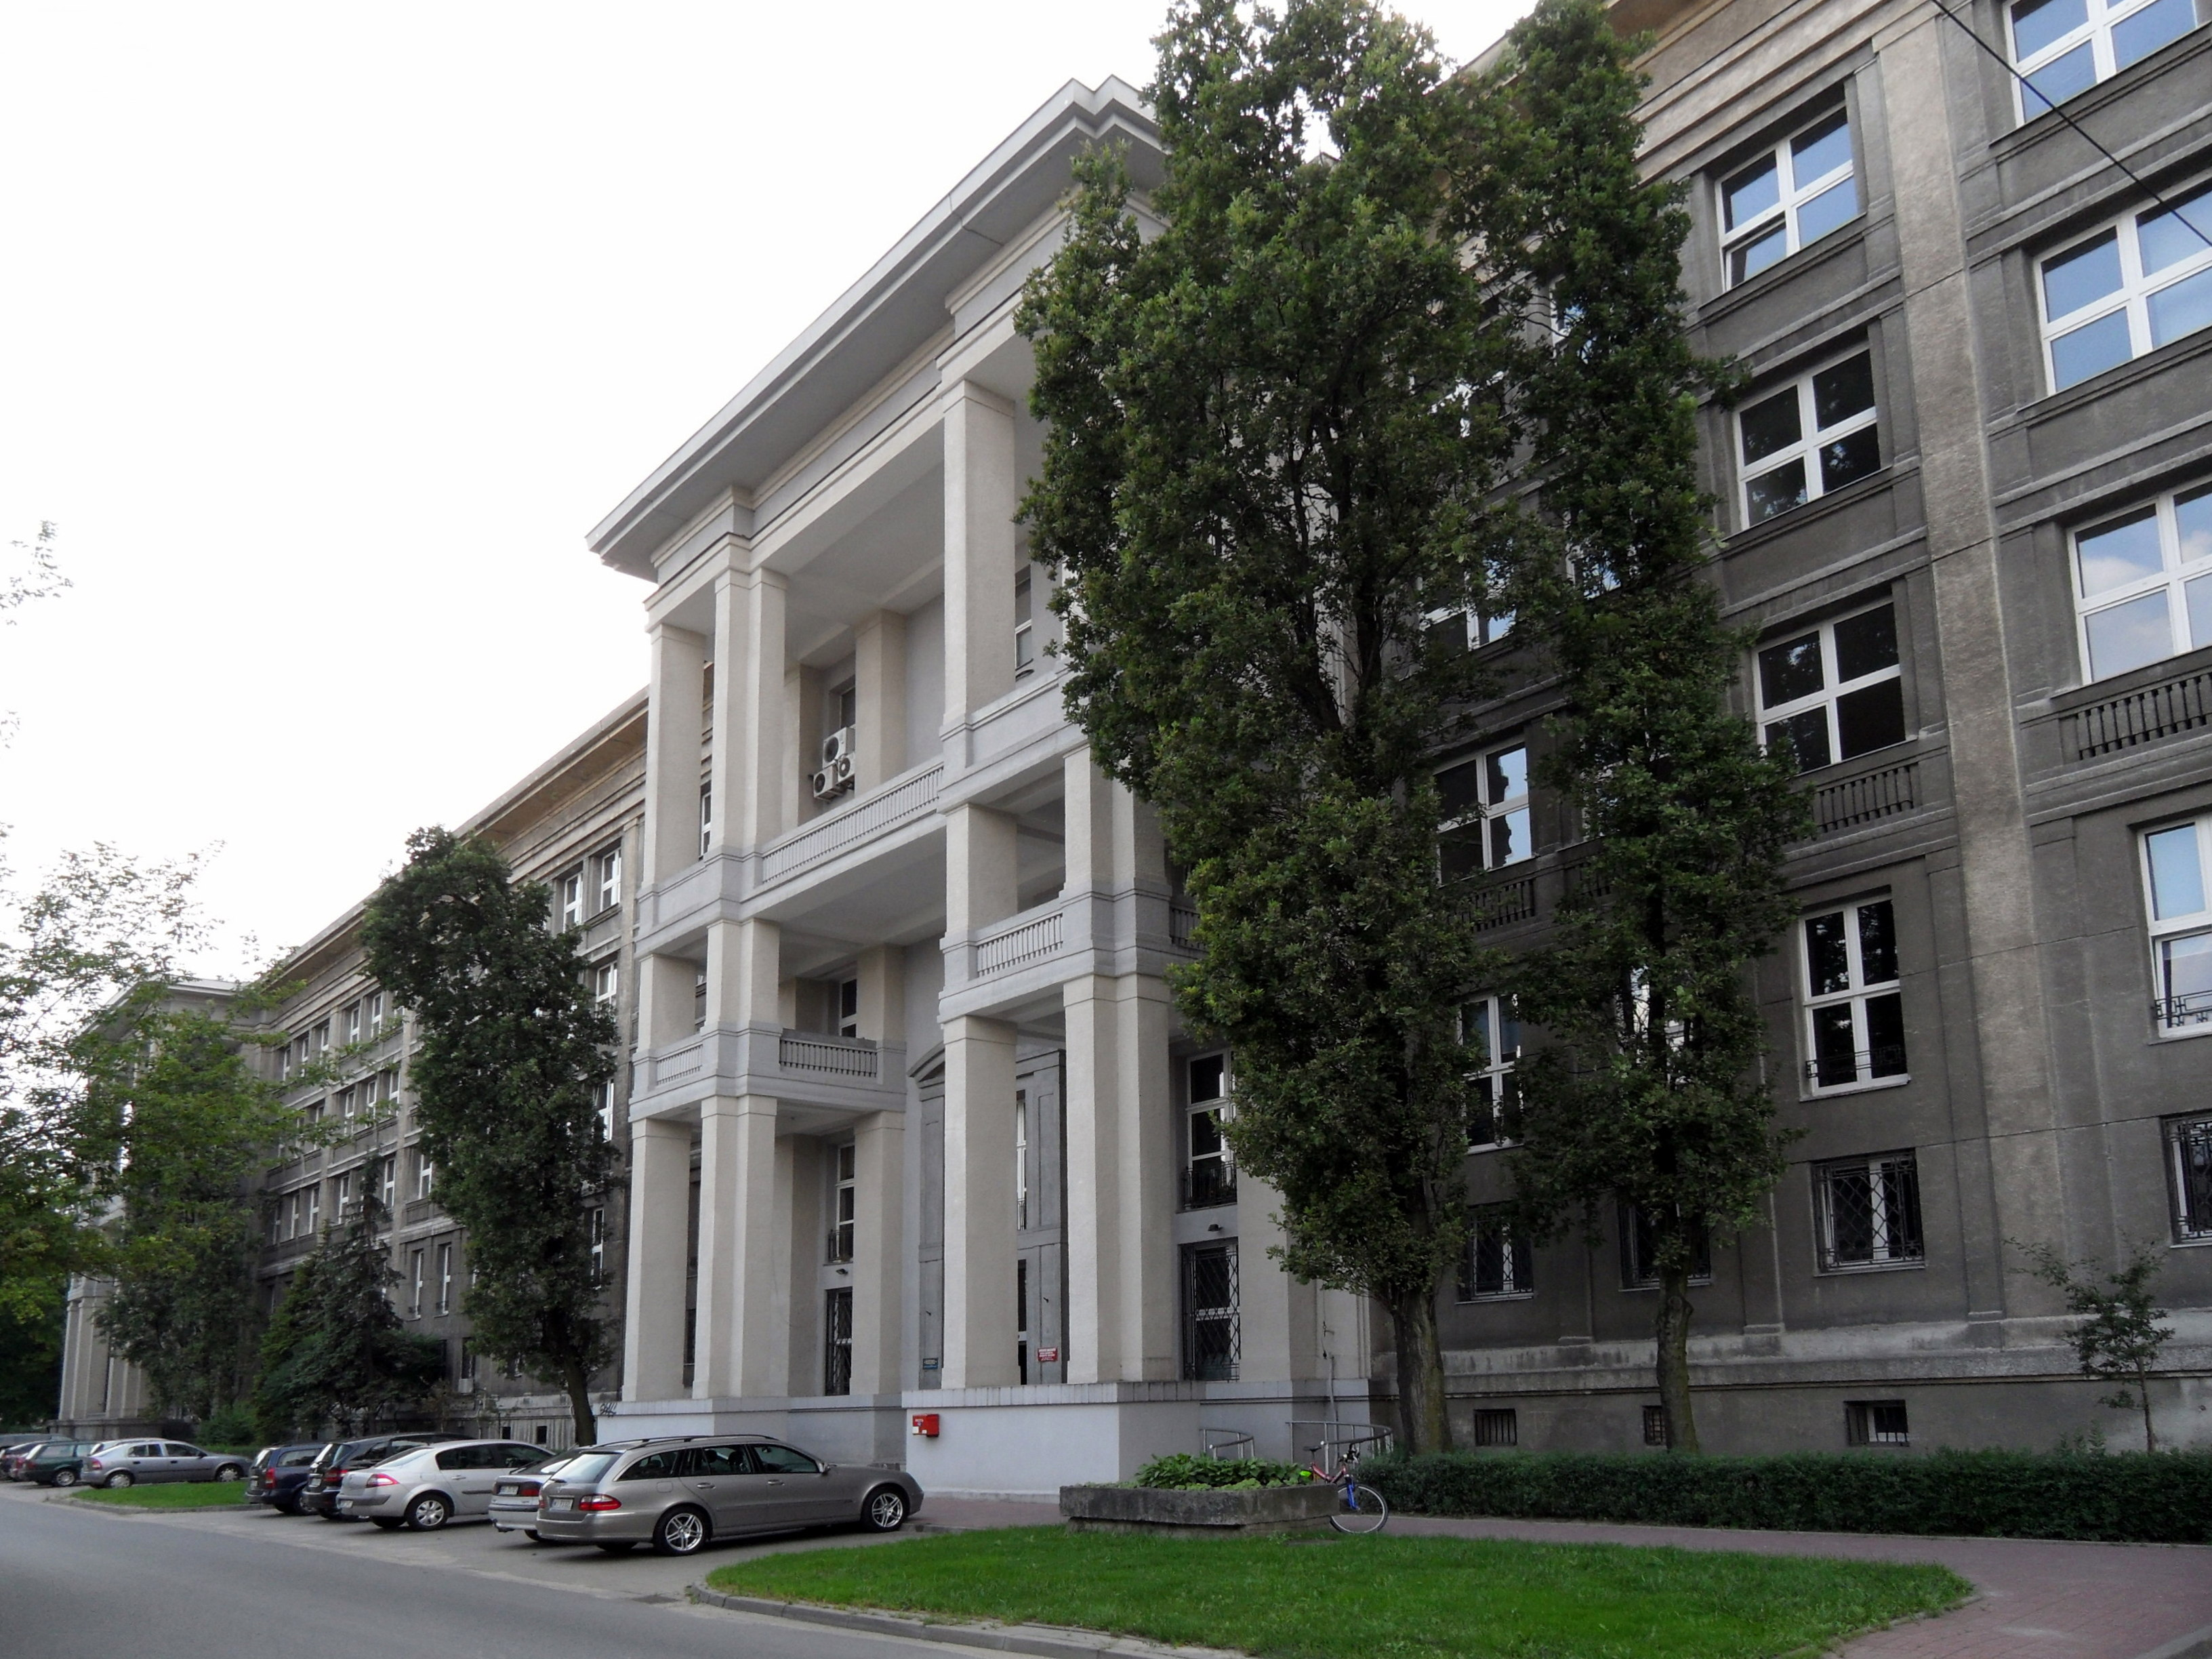
\includegraphics[height=0.6\textwidth]{images/mimuw.jpg}
		\caption{MIMUW (CC BY-SA 3.0 Krzysztof Dudzik \cite{wiki:mimuw})}
	\end{figure}
\end{frame}

\begin{frame}[c,plain]
	\begin{figure}
		\centering
		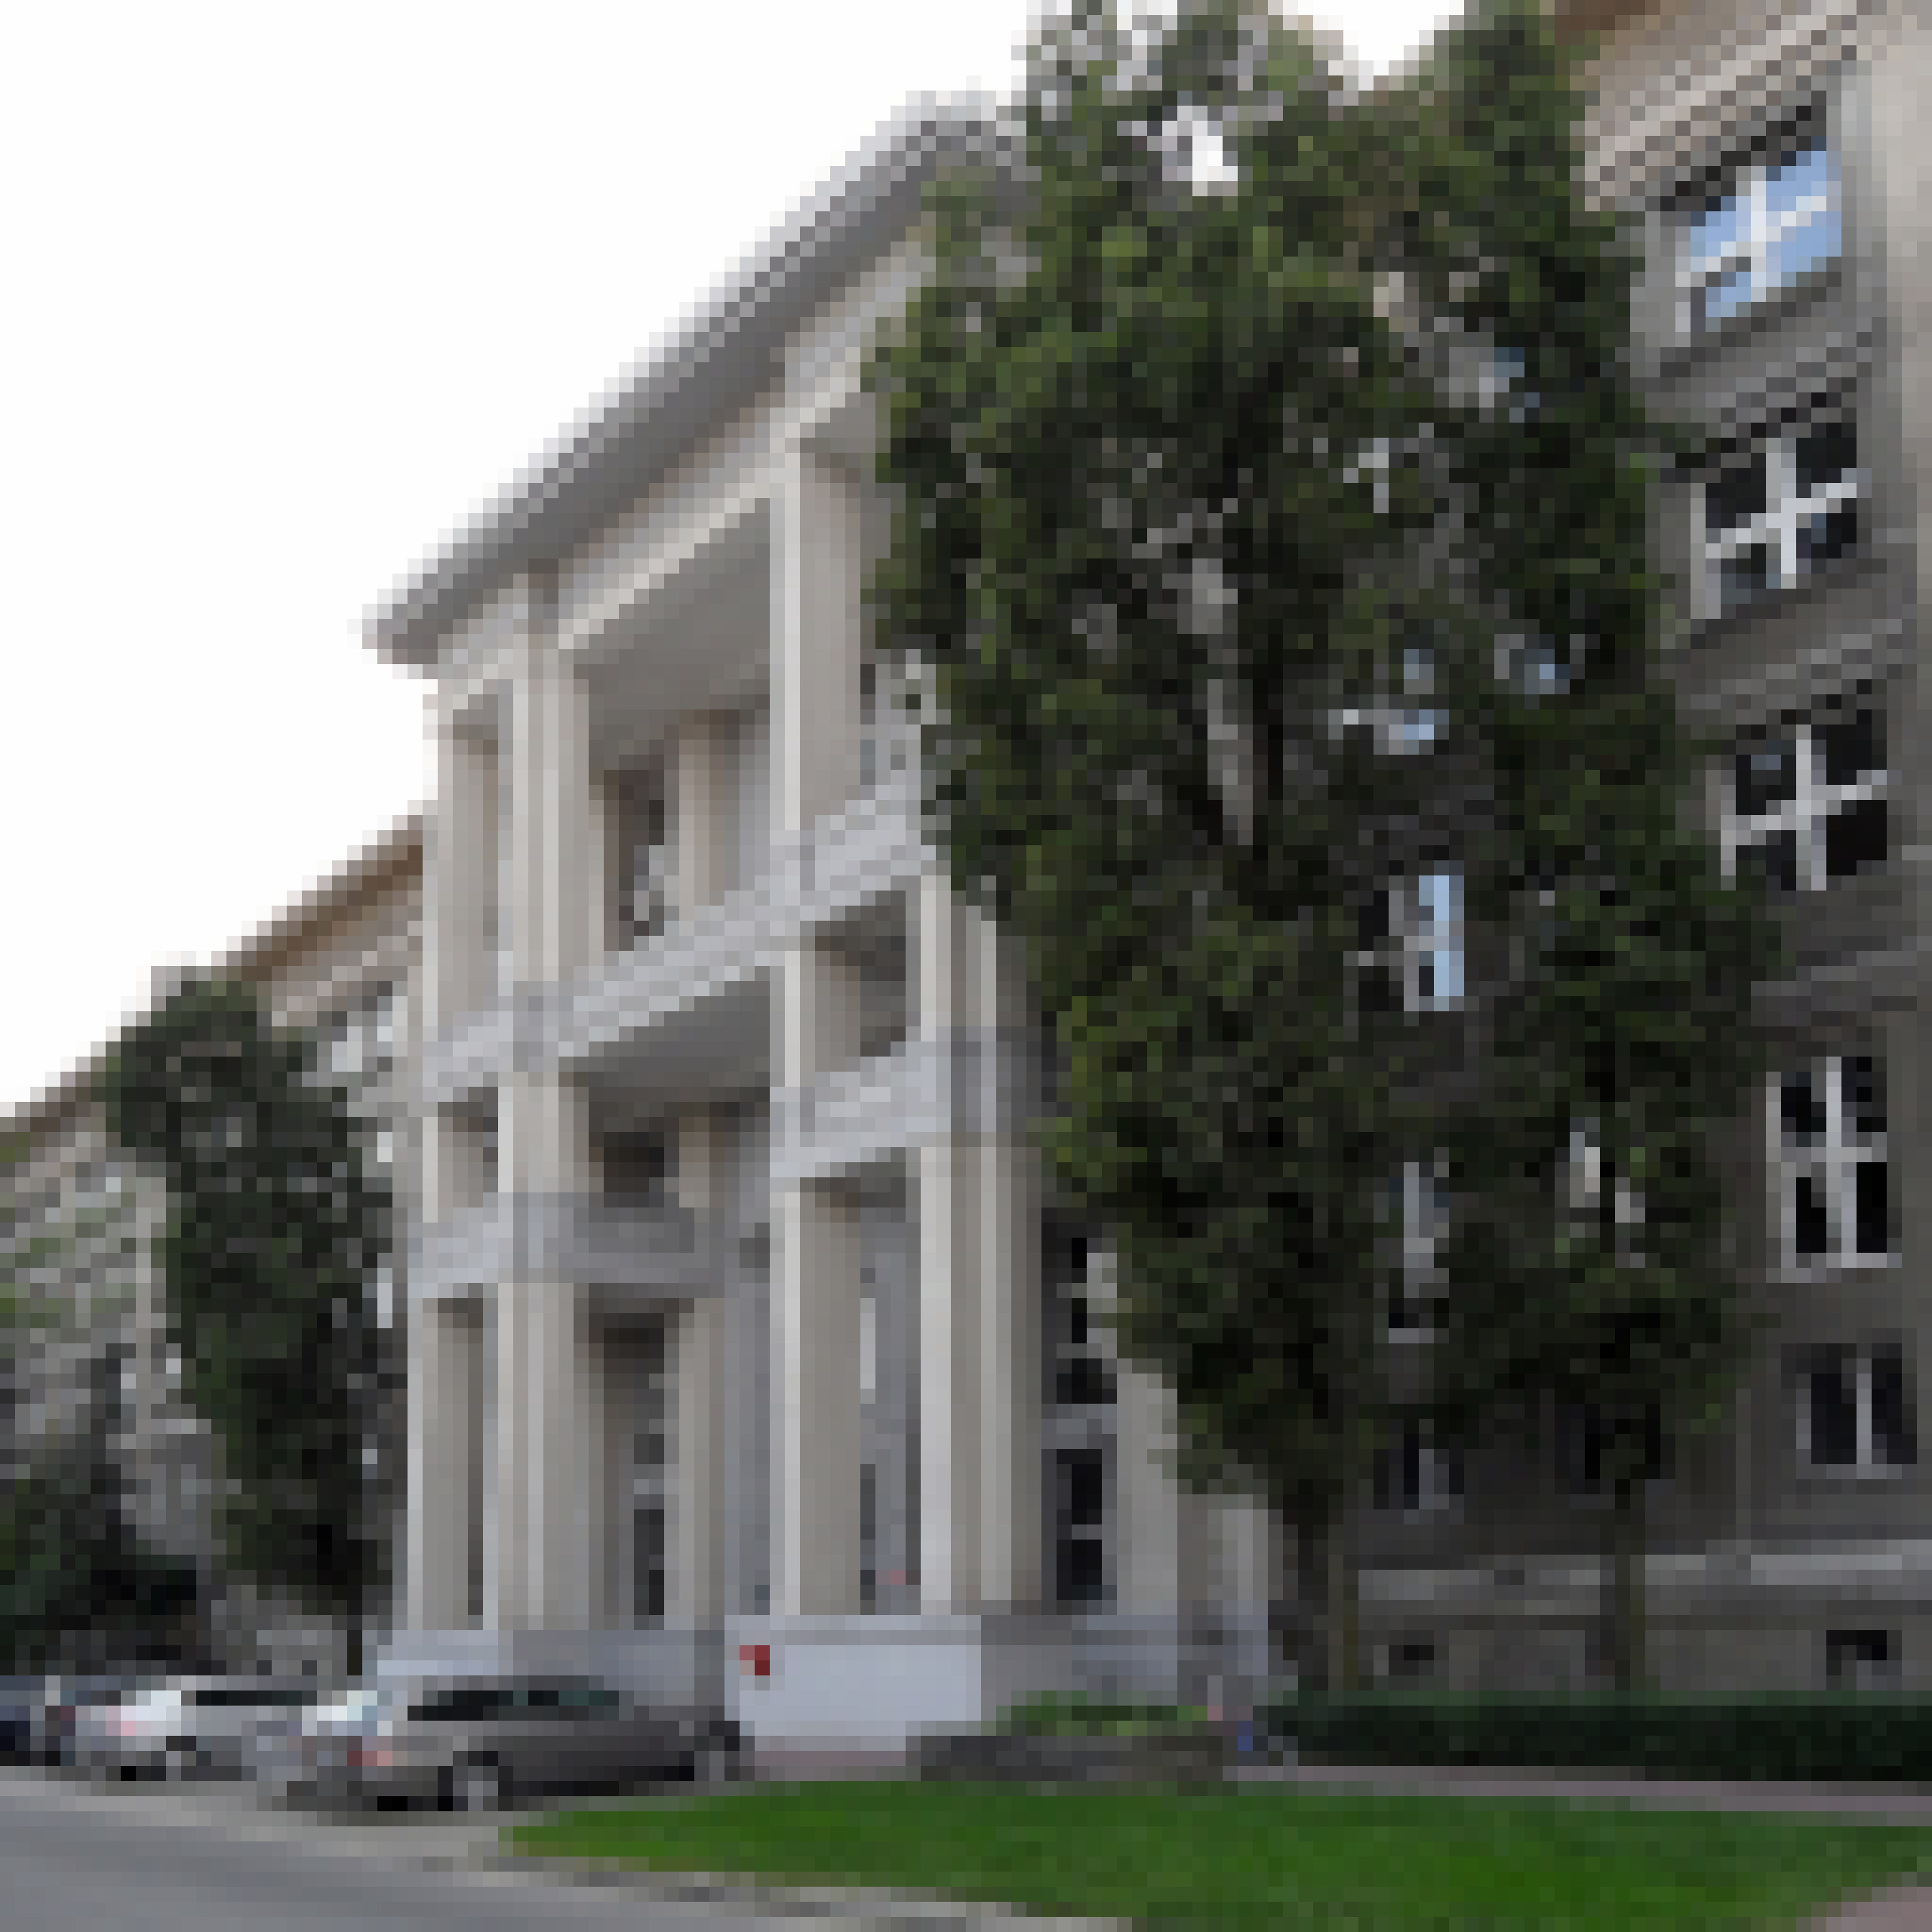
\includegraphics[height=0.6\textwidth]{images/mimuw-square-128-upscaled.png}
		\caption{Test image before compression, 128$\times$128 pixels.}
	\end{figure}
\end{frame}

\begin{frame}[c,plain]
	\vspace{5pt}
	\begin{figure}
		\centering
		\begin{tikzpicture}
			\fill[white] (-2,1) rectangle (9,0);
			
			\node (rgb) at (3.5, 3.8) {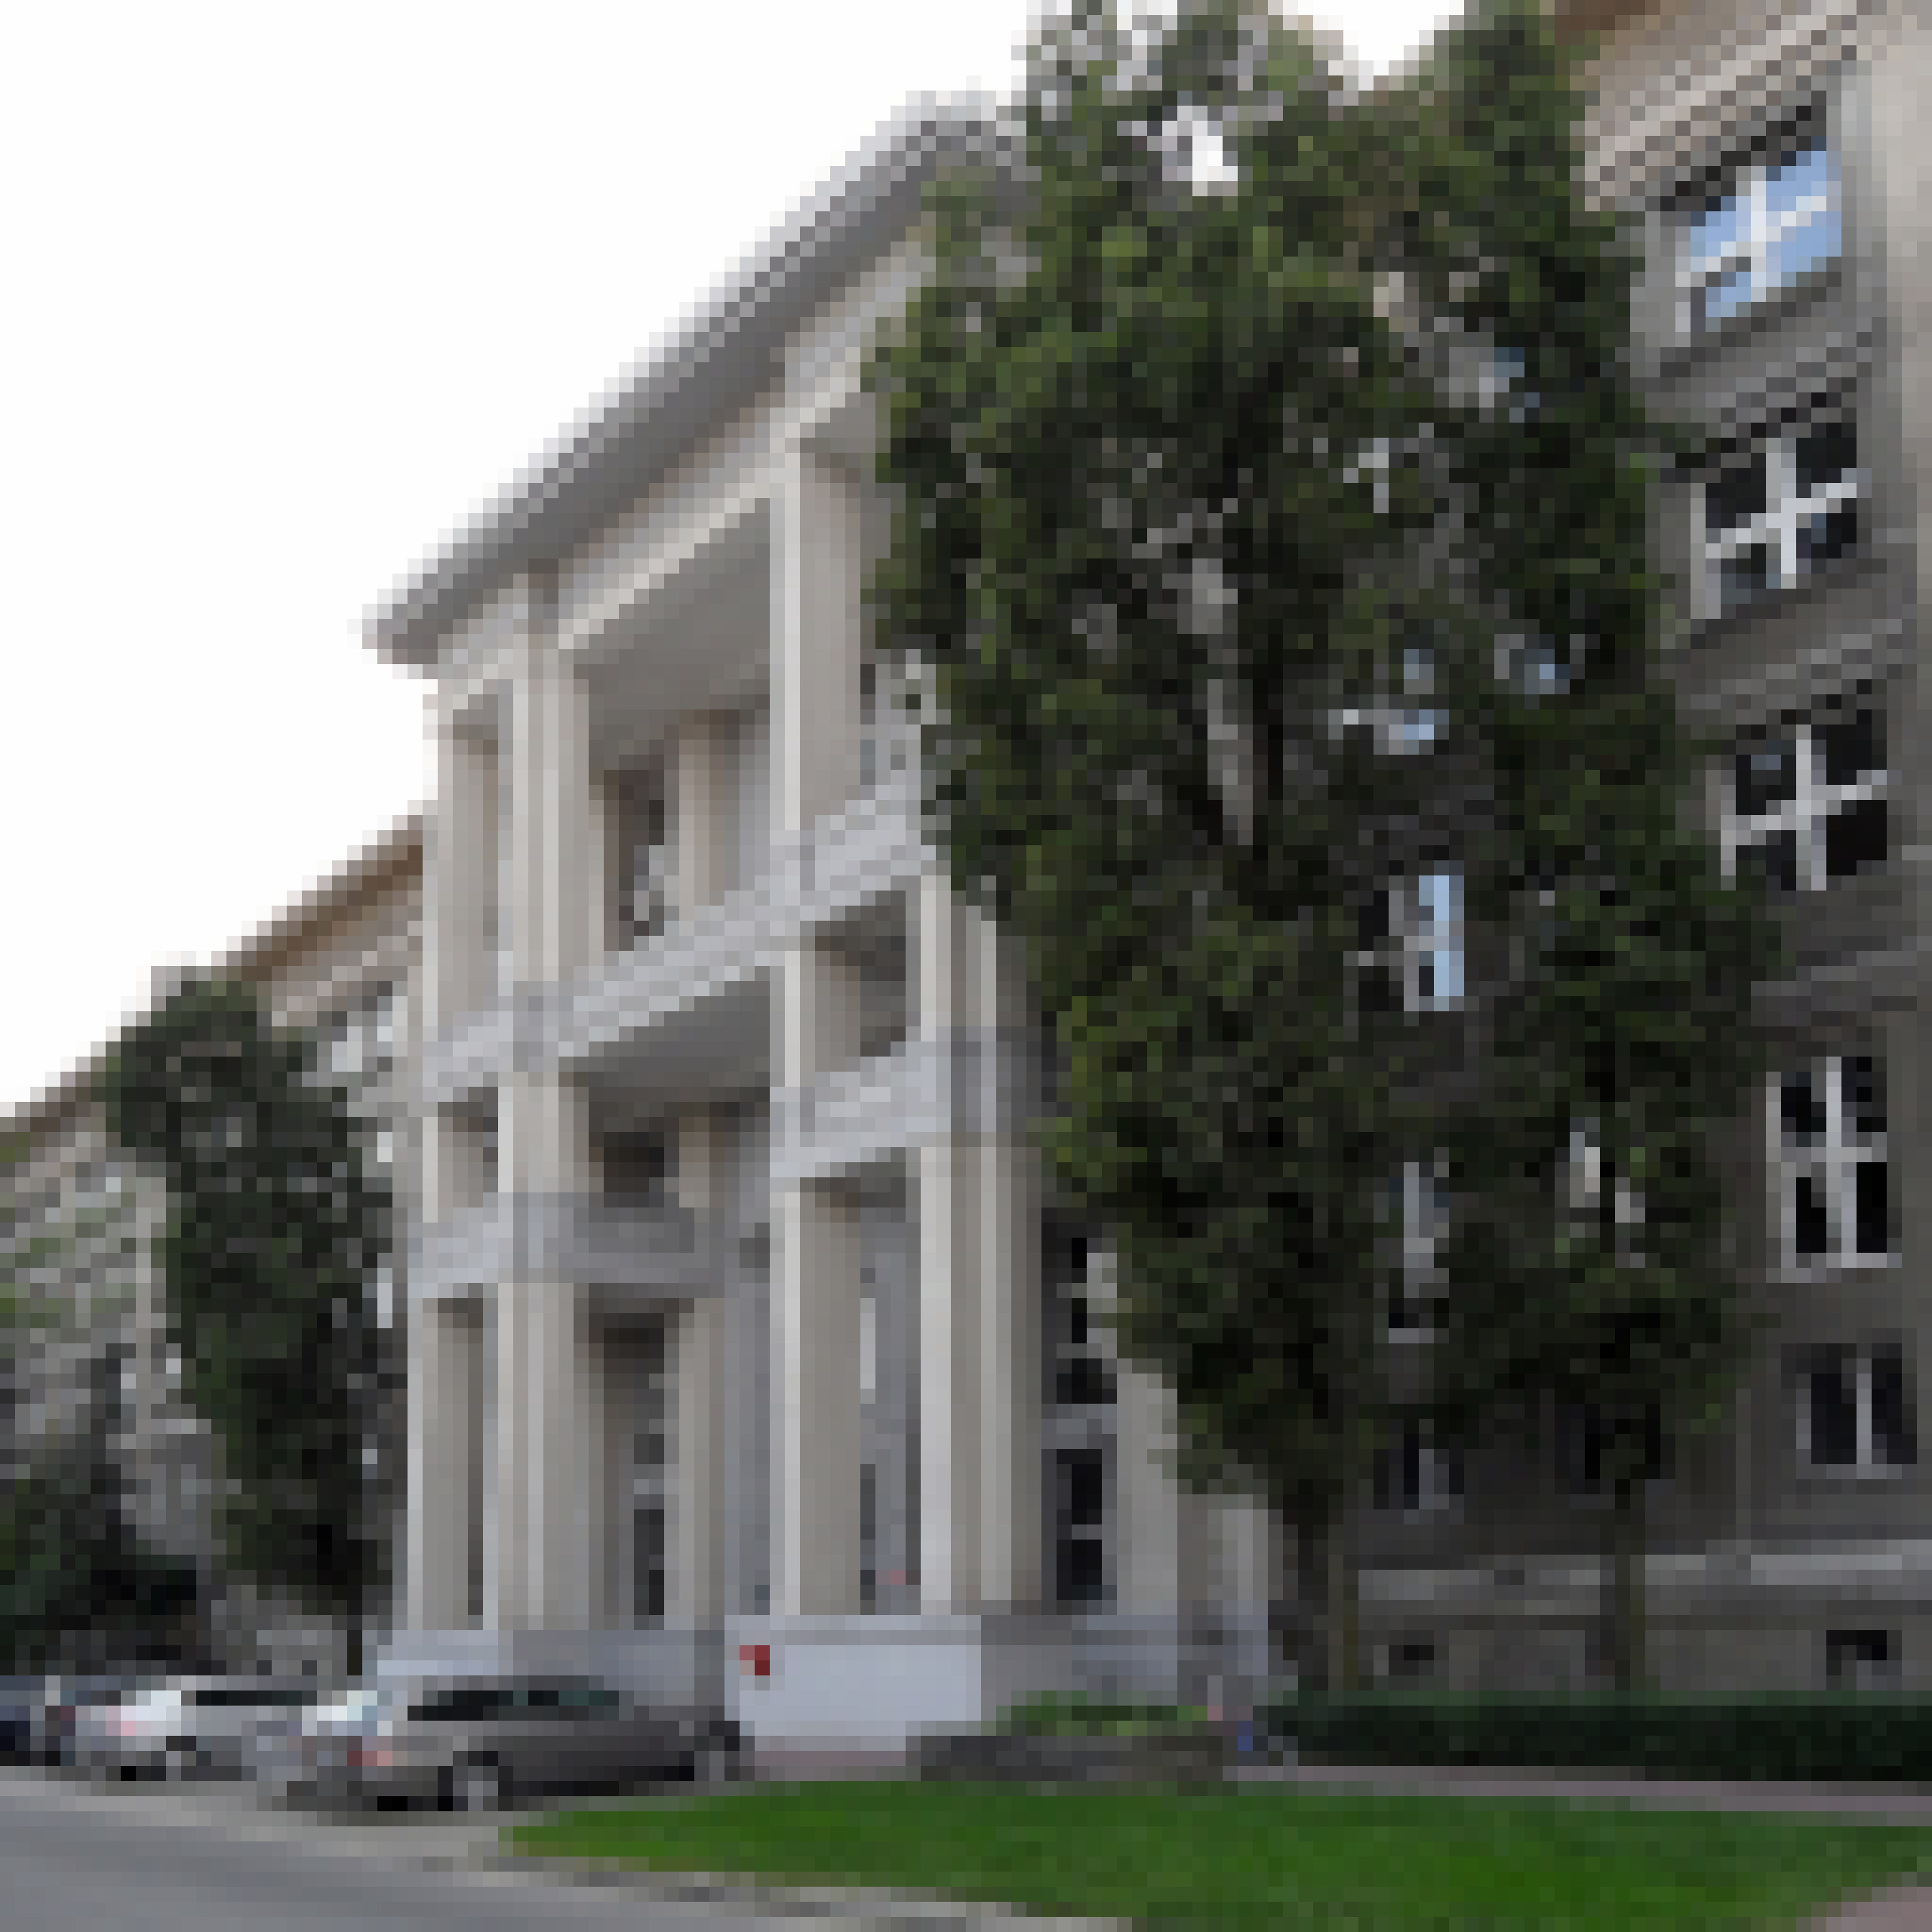
\includegraphics[height=0.25\textwidth]{images/mimuw-square-128-upscaled.png}};
			\node (red) at (0,0) {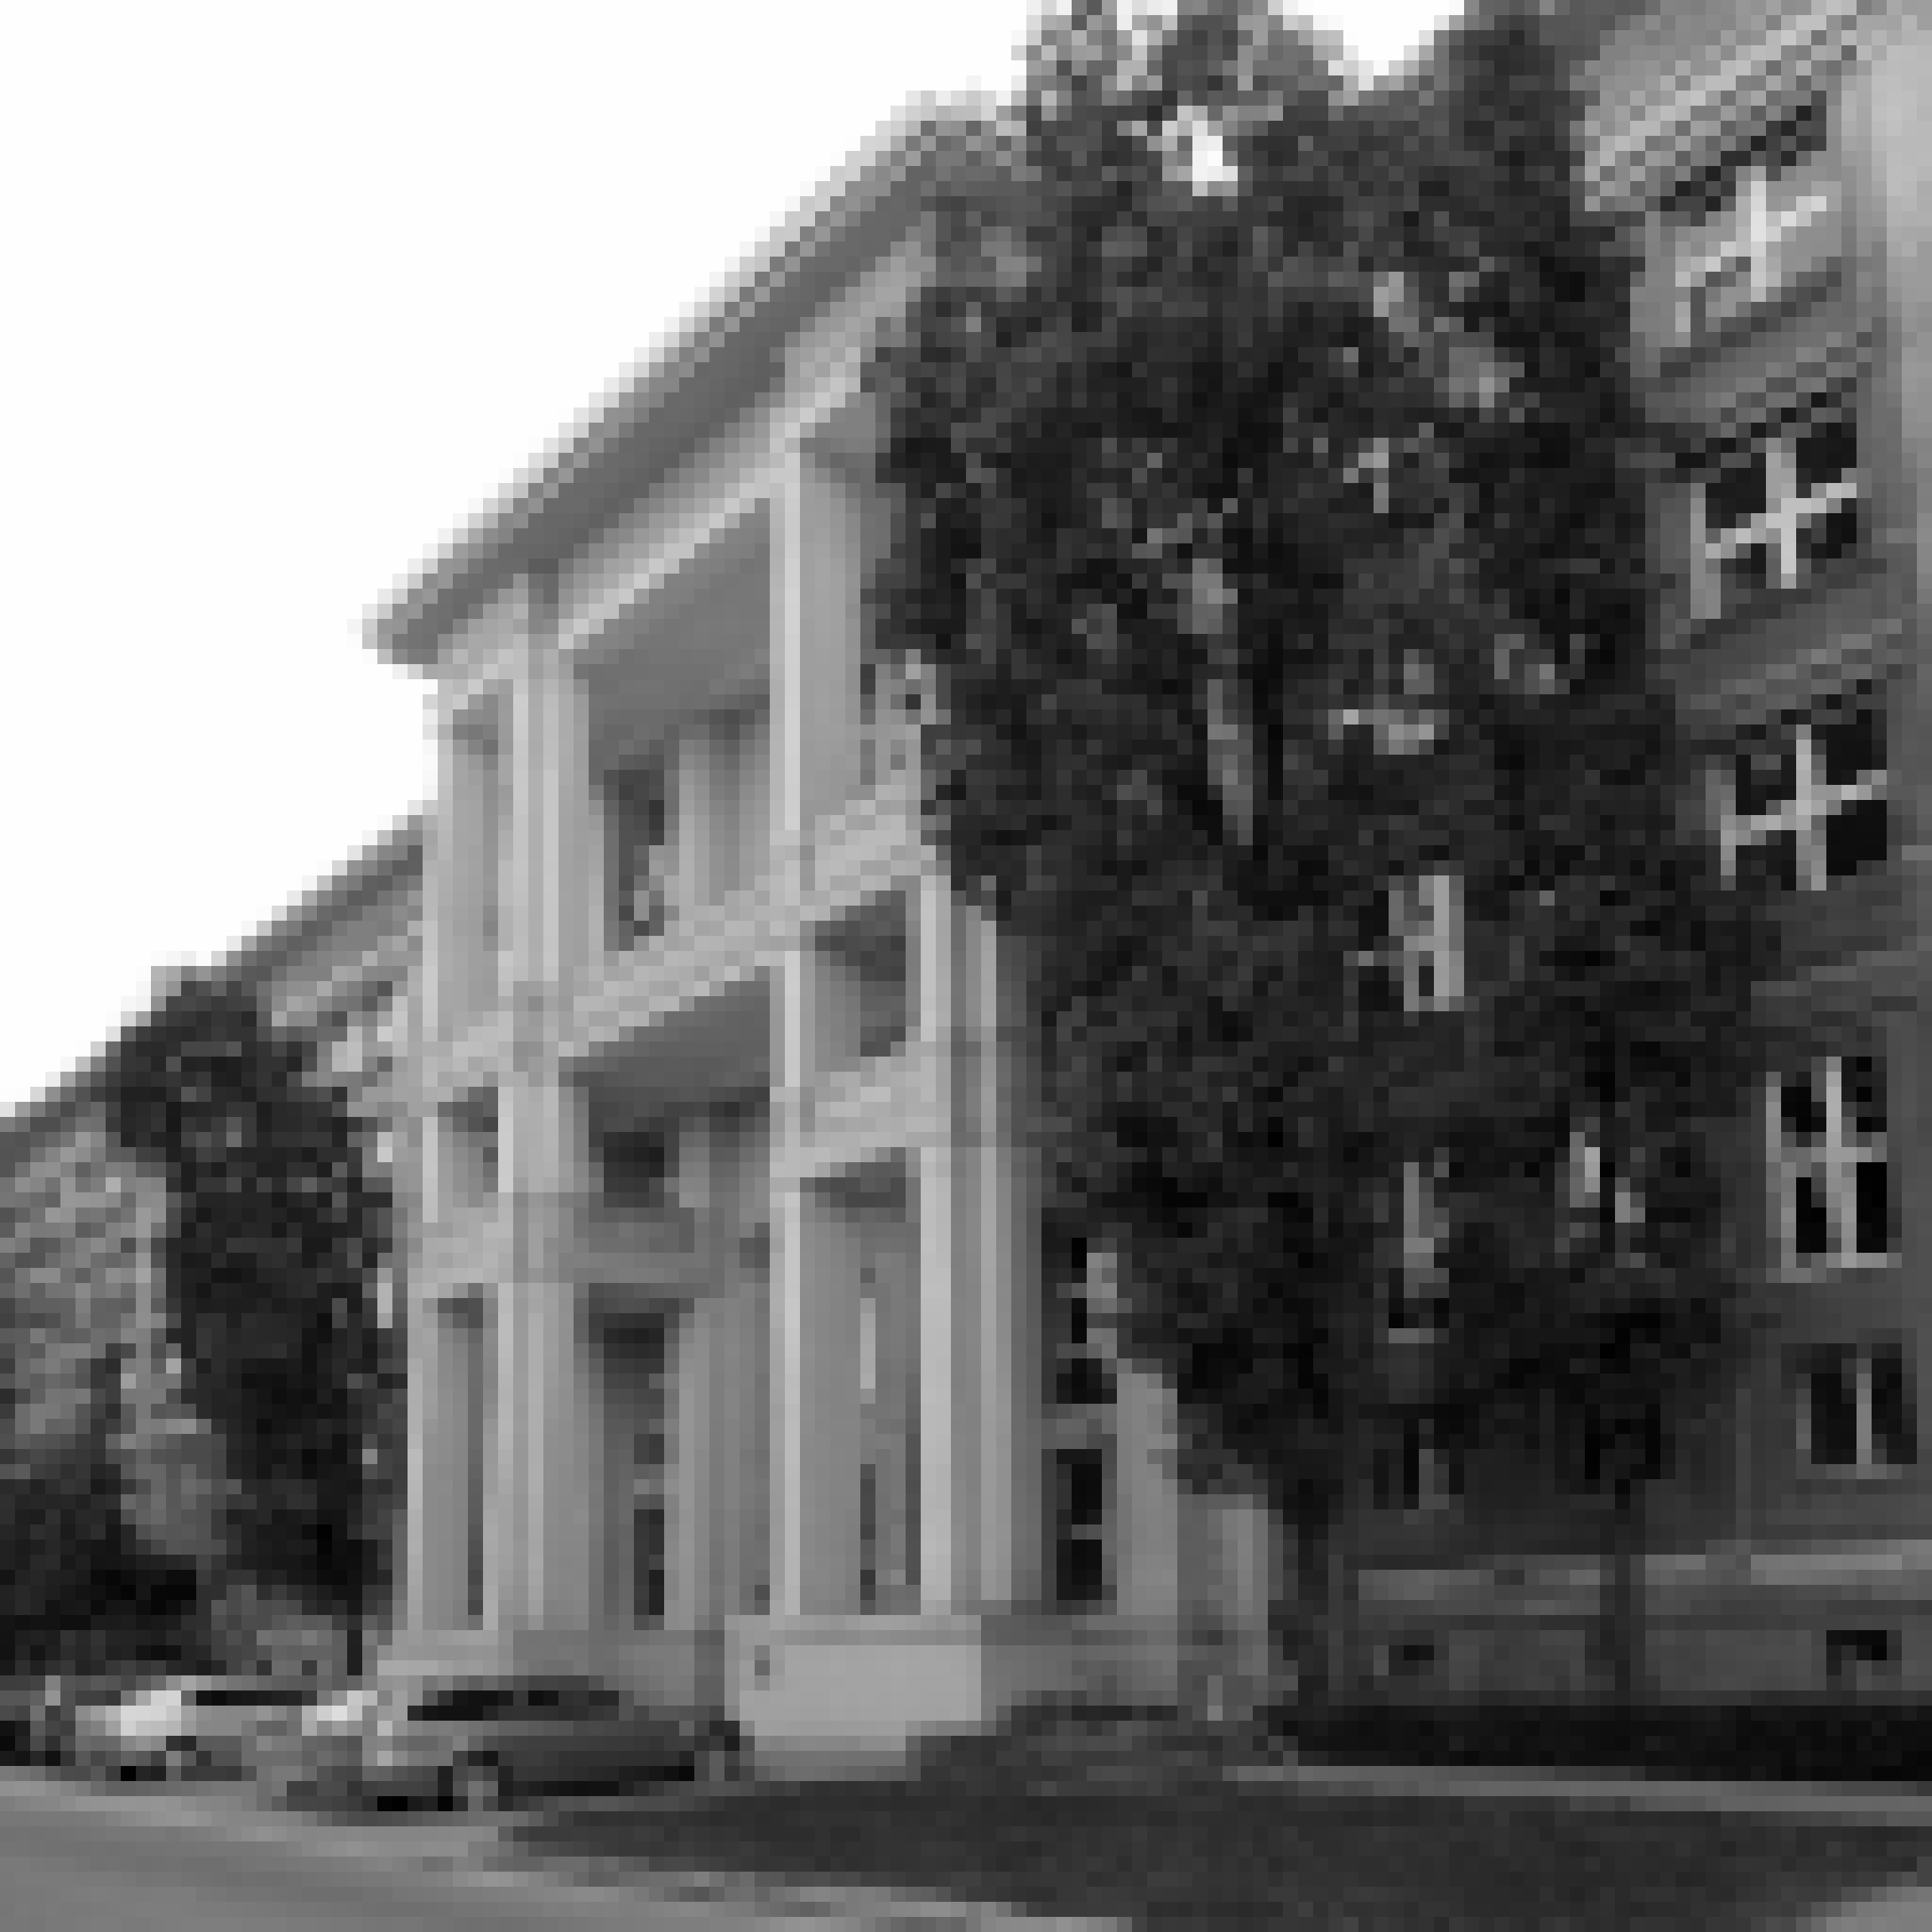
\includegraphics[height=0.25\textwidth]{images/mimuw-square-128-rgb-red-upscaled.png}};
			\node (green) at (3.5,0) {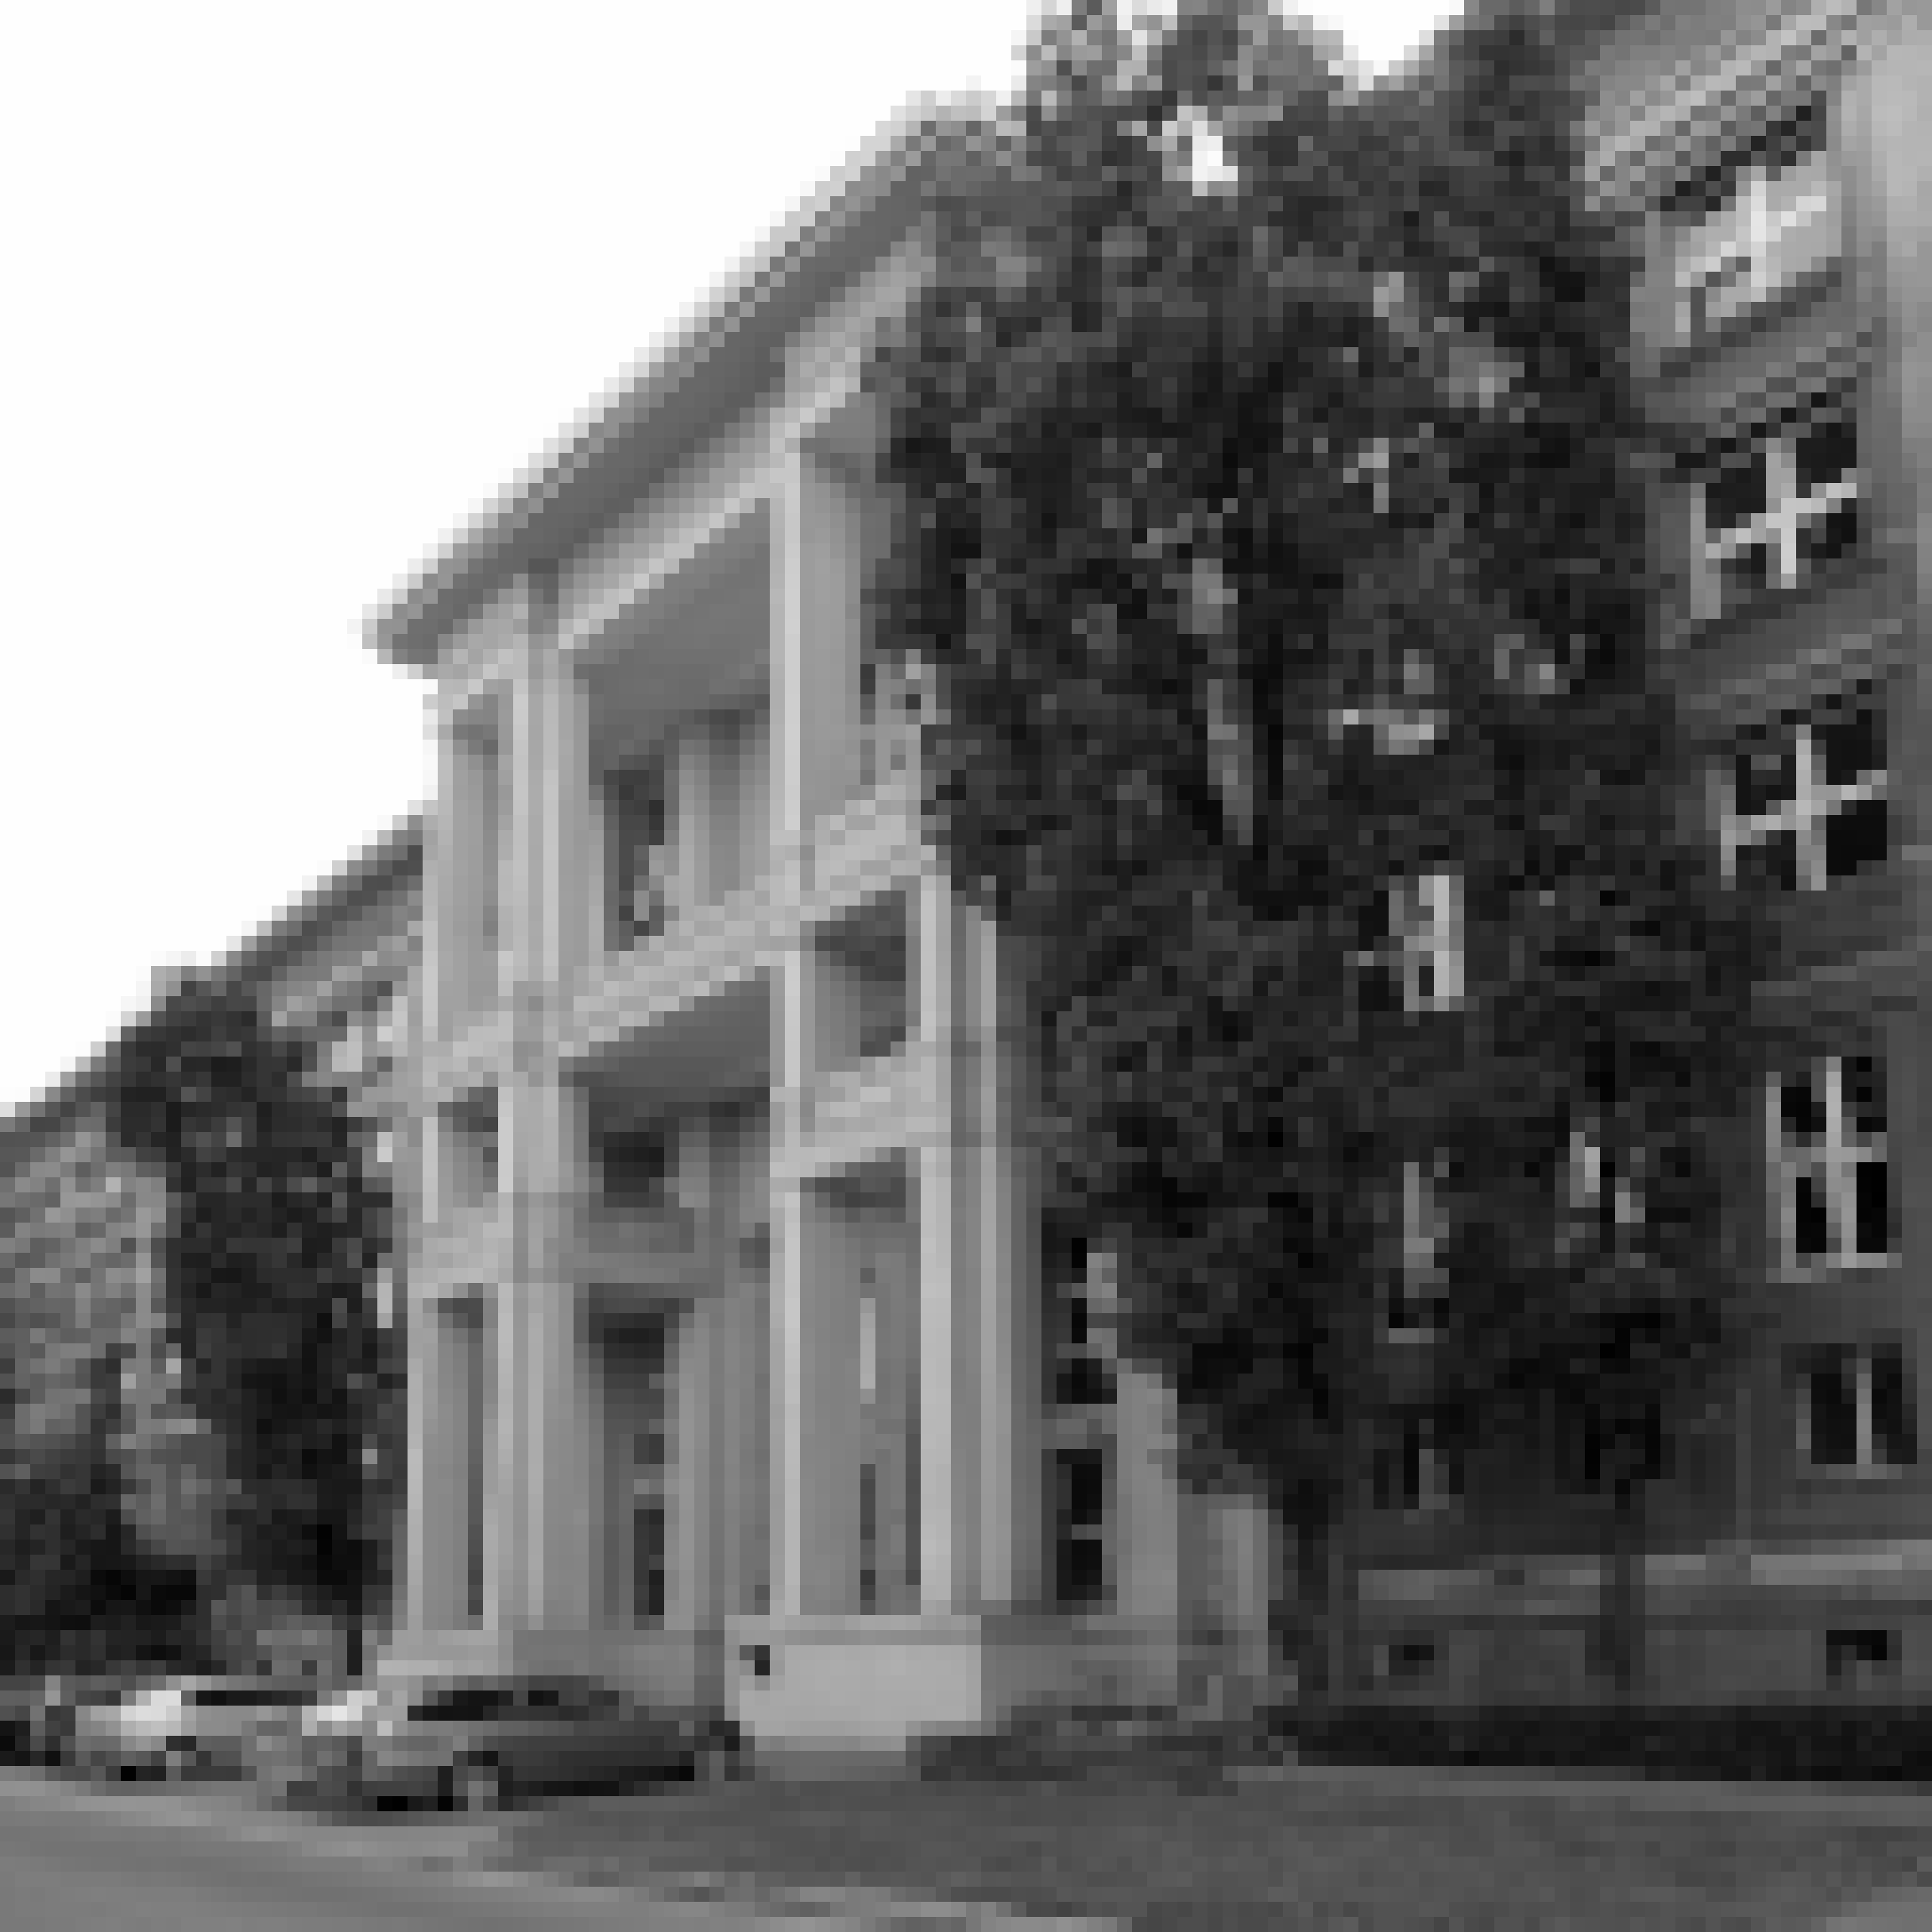
\includegraphics[height=0.25\textwidth]{images/mimuw-square-128-rgb-green-upscaled.png}};
			\node (blue) at (7,0) {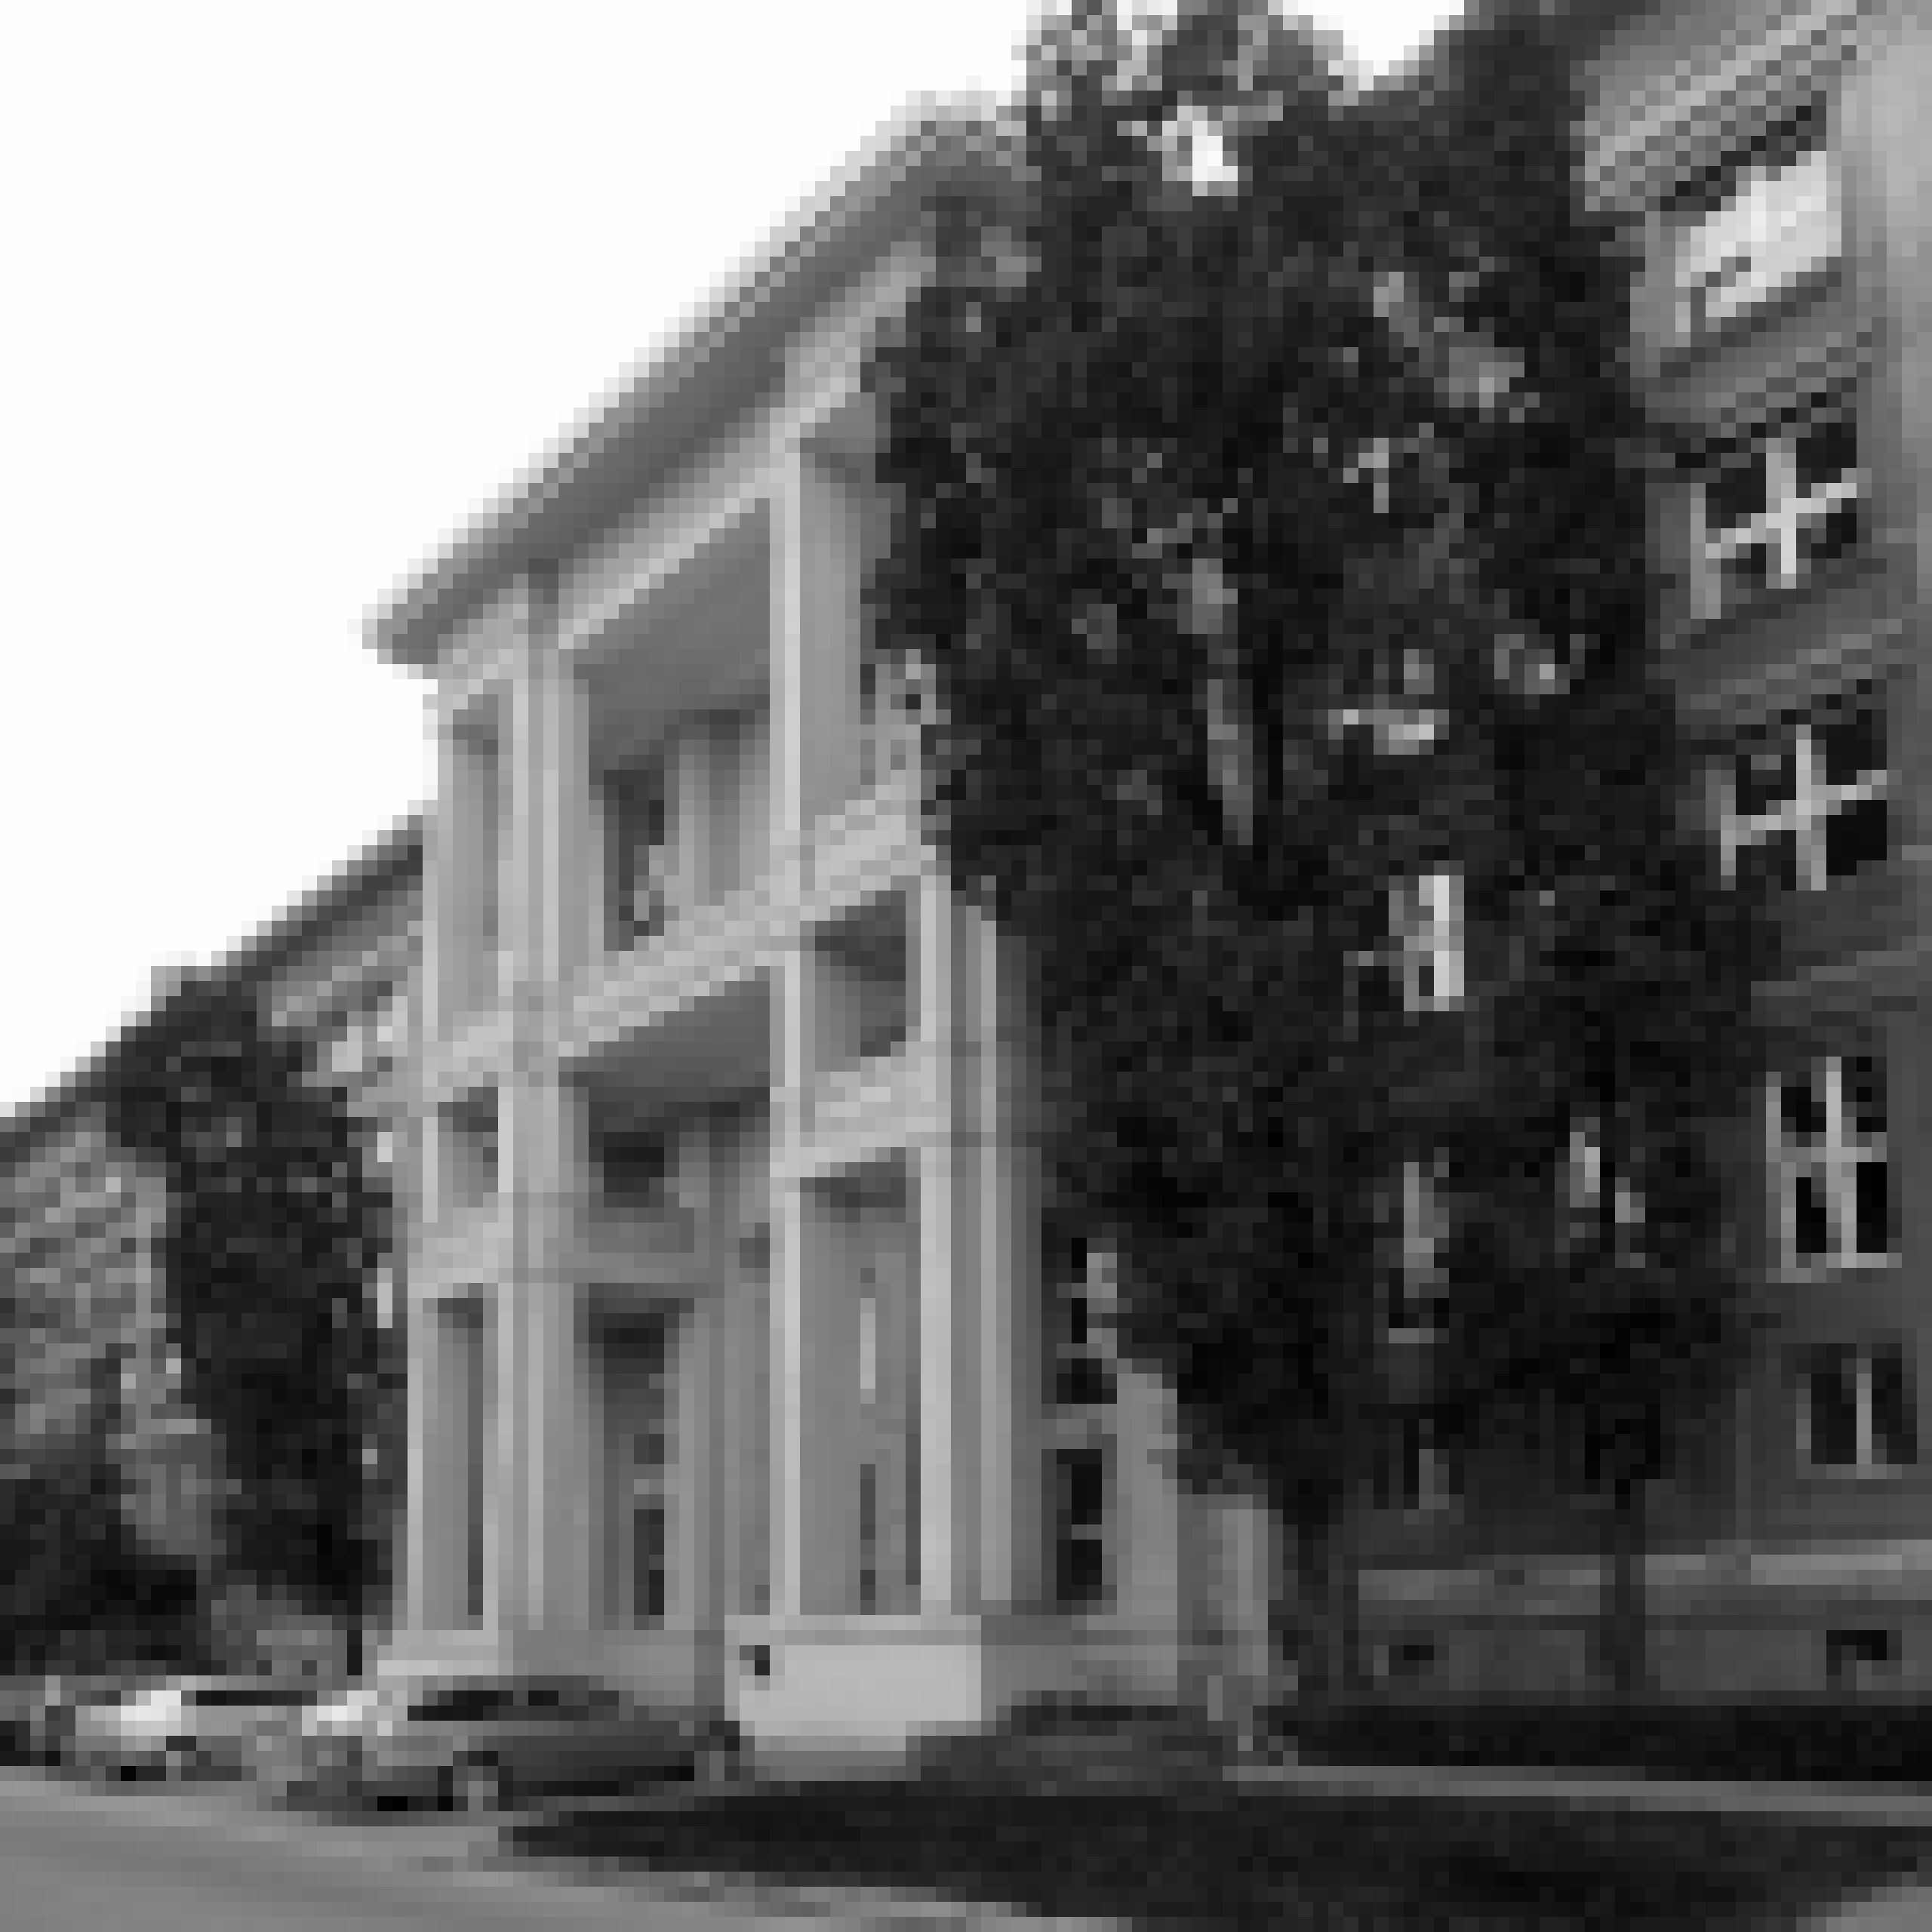
\includegraphics[height=0.25\textwidth]{images/mimuw-square-128-rgb-blue-upscaled.png}};
		
			\node[below] at (red.south) {\textsc{r}};
			\node[below] at (green.south) {\textsc{g}};
			\node[below] at (blue.south) {\textsc{b}};
			
			\draw [<-, shorten >=3pt, shorten <=3pt] (red) -- (rgb);
			\draw [<-, shorten >=3pt, shorten <=3pt] (green) -- (rgb);
			\draw [<-, shorten >=3pt, shorten <=3pt] (blue) -- (rgb);

			% Annotations			
			\pause

			\definecolor{mygreen}{rgb}{0,0.8,0}
			\definecolor{myblue}{rgb}{0.2,0.2,1}

			\draw[myblue,thick] ($ (rgb) + (1.11,1.08) $) circle (0.3);
			\draw[myblue,thick] ($ (blue) + (1.11,1.08) $) circle (0.3);
			
			\draw[mygreen,thick,rounded corners] ($ (rgb) + (-0.6,-0.8) $) rectangle ($ (rgb) + (1.5,-1.5) $);
			\draw[mygreen,thick,rounded corners] ($ (green) + (-0.6,-0.8) $) rectangle ($ (green) + (1.5,-1.5) $);
			
			\node[align=left] at (7.3,3.8) {
				\footnotesize Channel pixel has greater \\
				\footnotesize value if source image pixel \\
				\footnotesize matches channel color.};
		\end{tikzpicture}
		\caption{Test image decomposed into RGB channels.}
	\end{figure}
\end{frame}

\begin{frame}[c,plain]
	\vspace{5pt}
	\begin{figure}
		\centering
		\begin{tikzpicture}
			\node (ycbcr) at (3.5, 3.8) {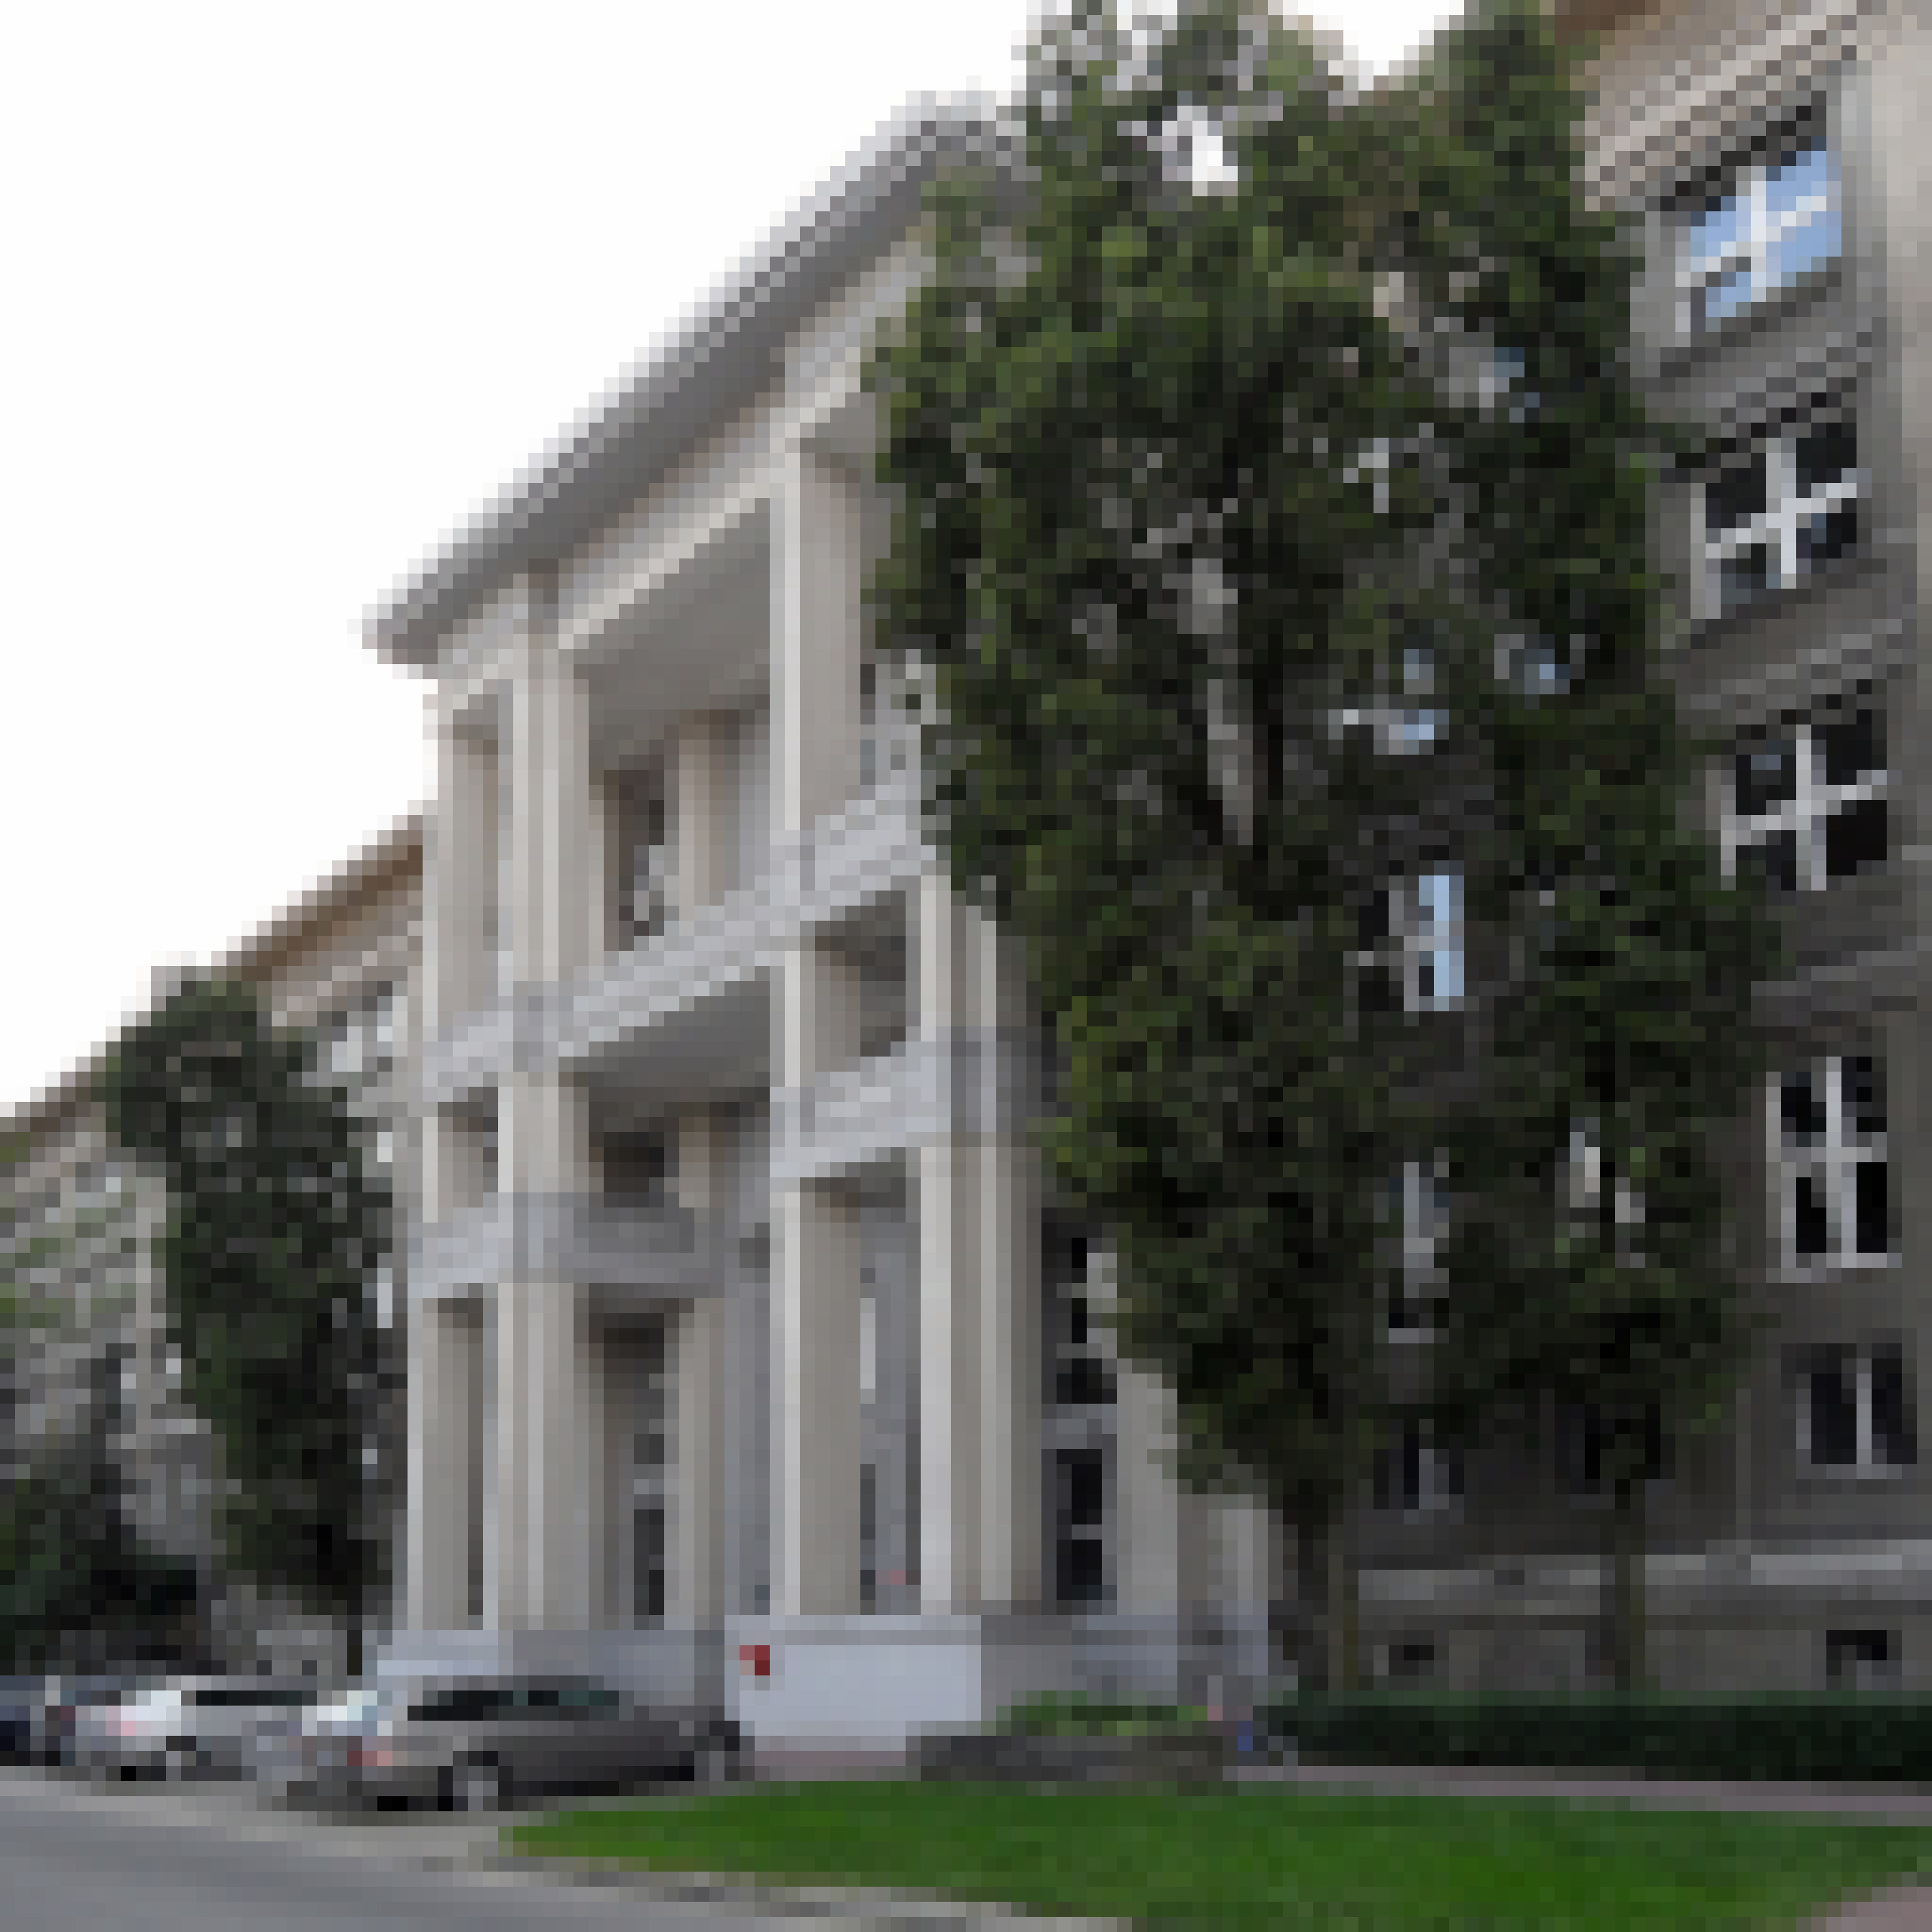
\includegraphics[height=0.25\textwidth]{images/mimuw-square-128-upscaled.png}};
			\node (luma) at (0,0) {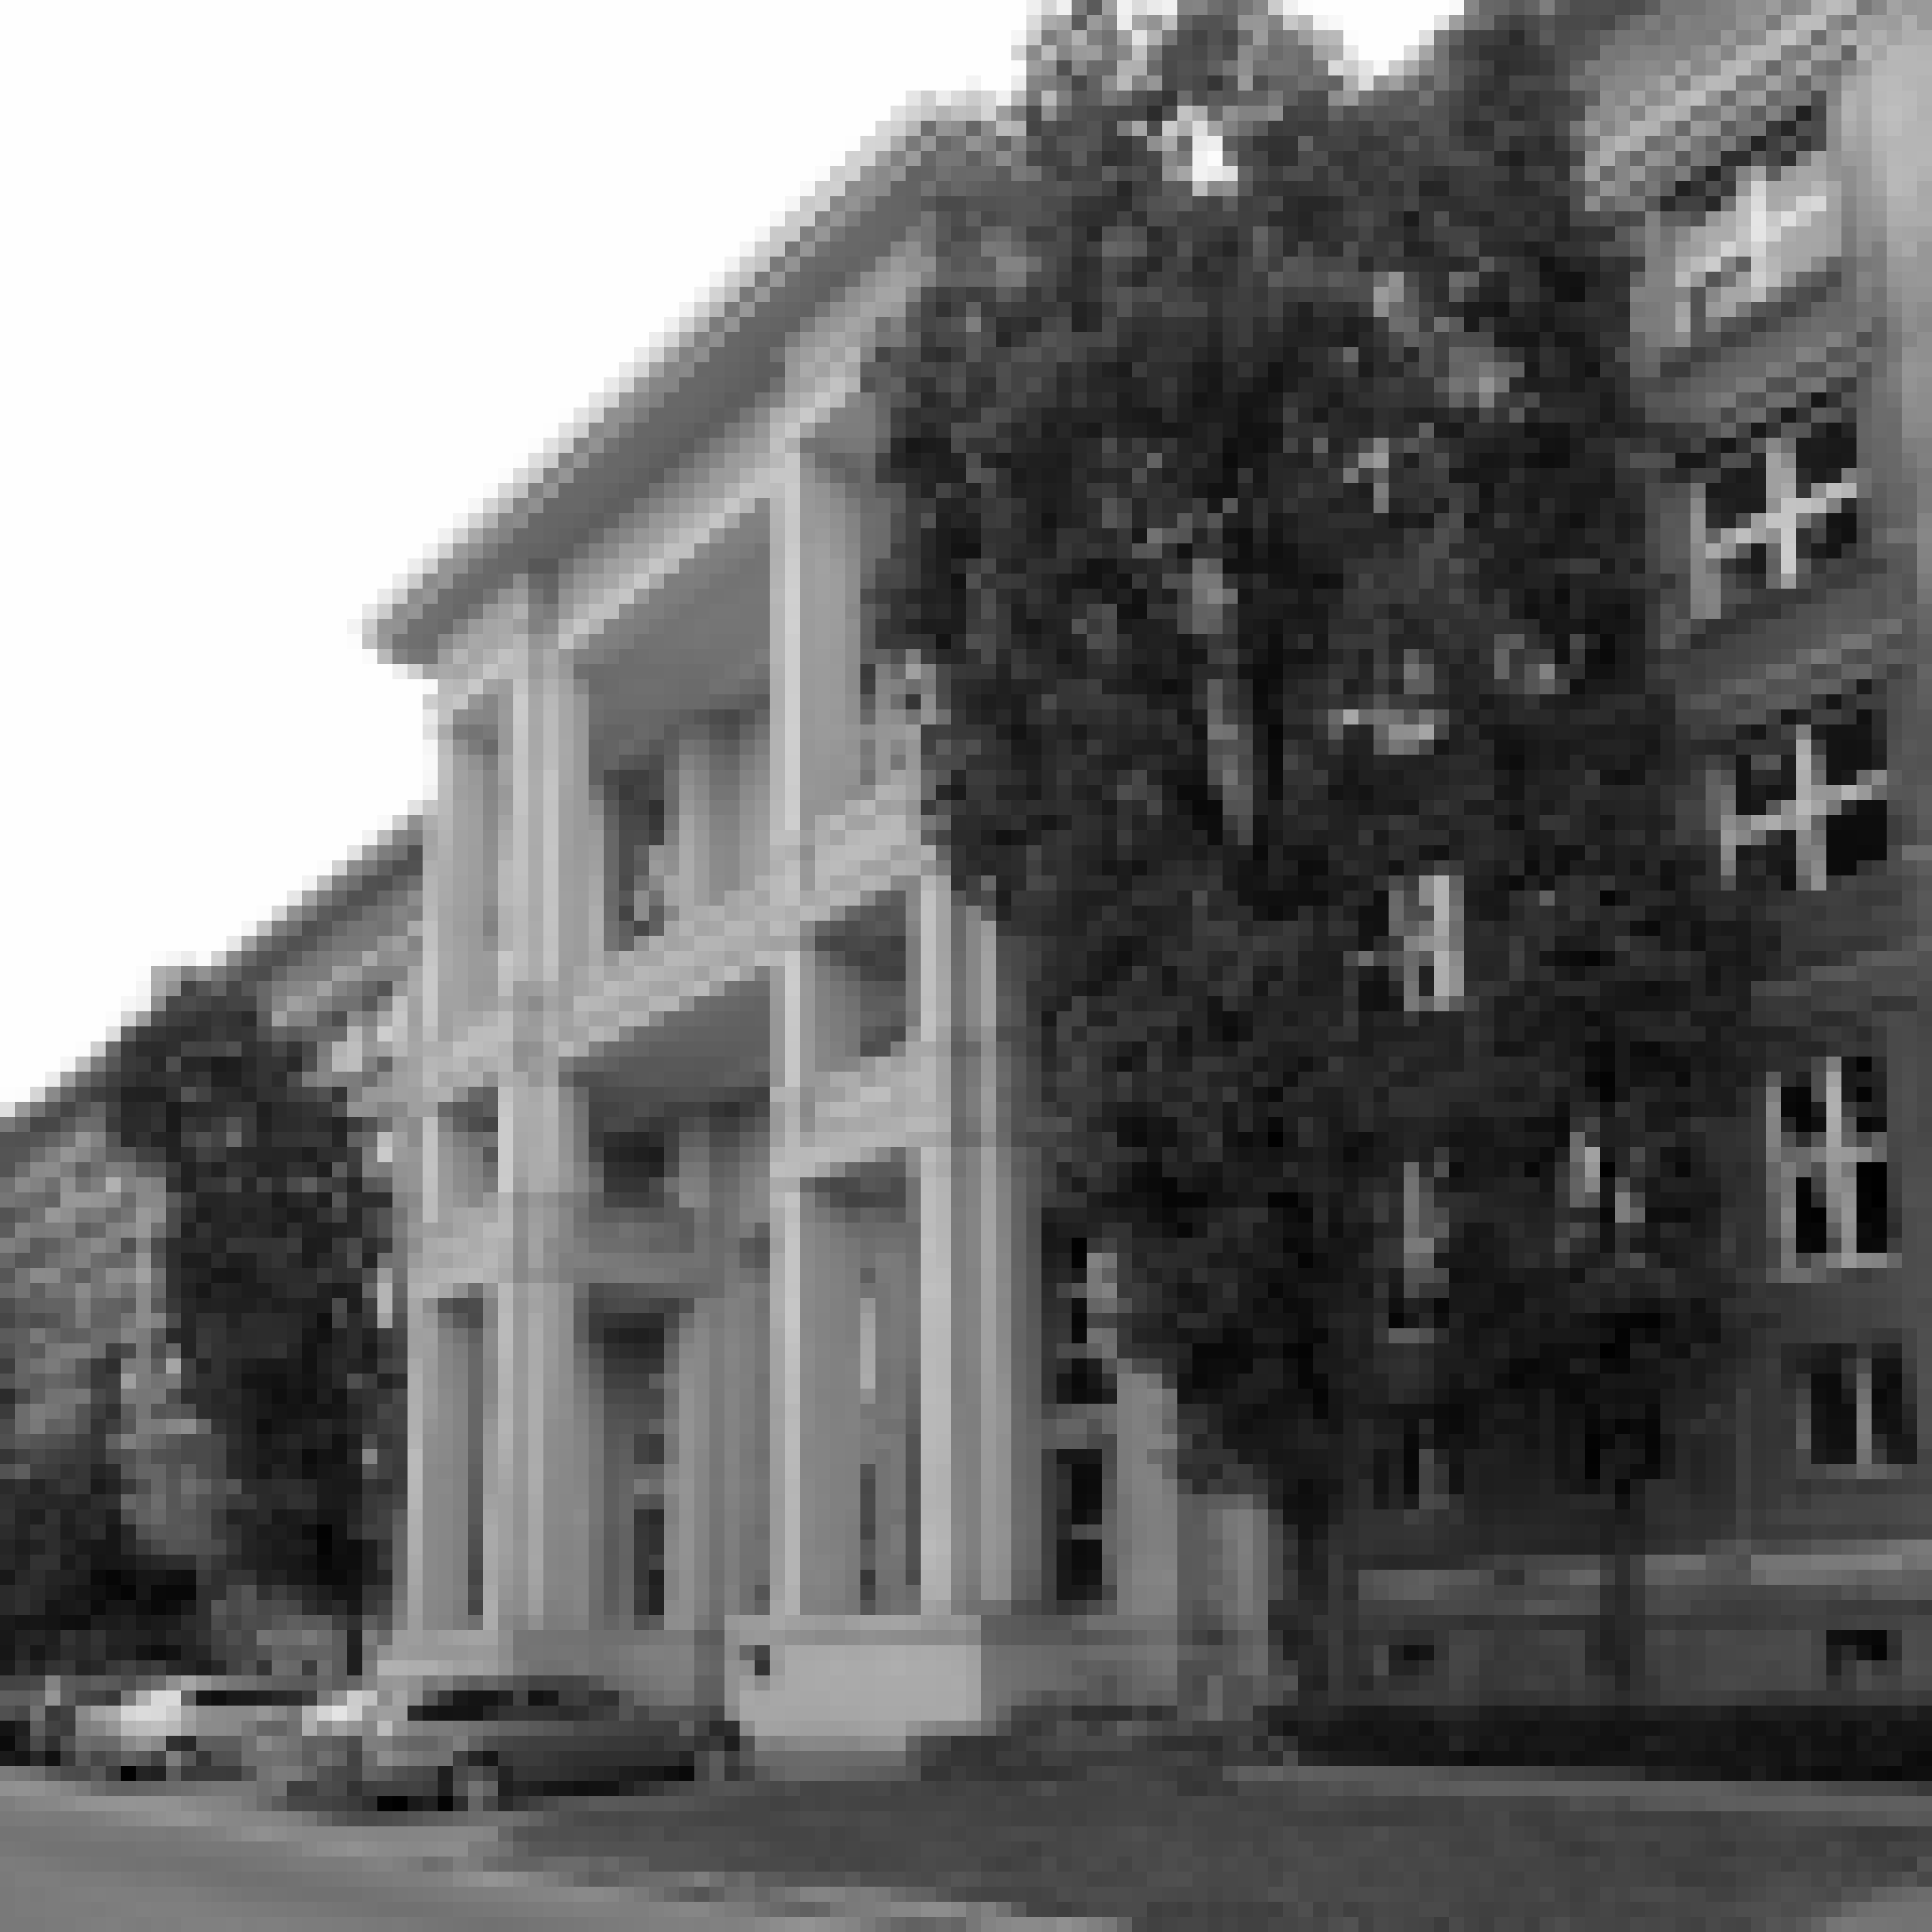
\includegraphics[height=0.25\textwidth]{images/mimuw-square-128-ycbcr-luma-upscaled.png}};
			\node (blueness) at (3.5,0) {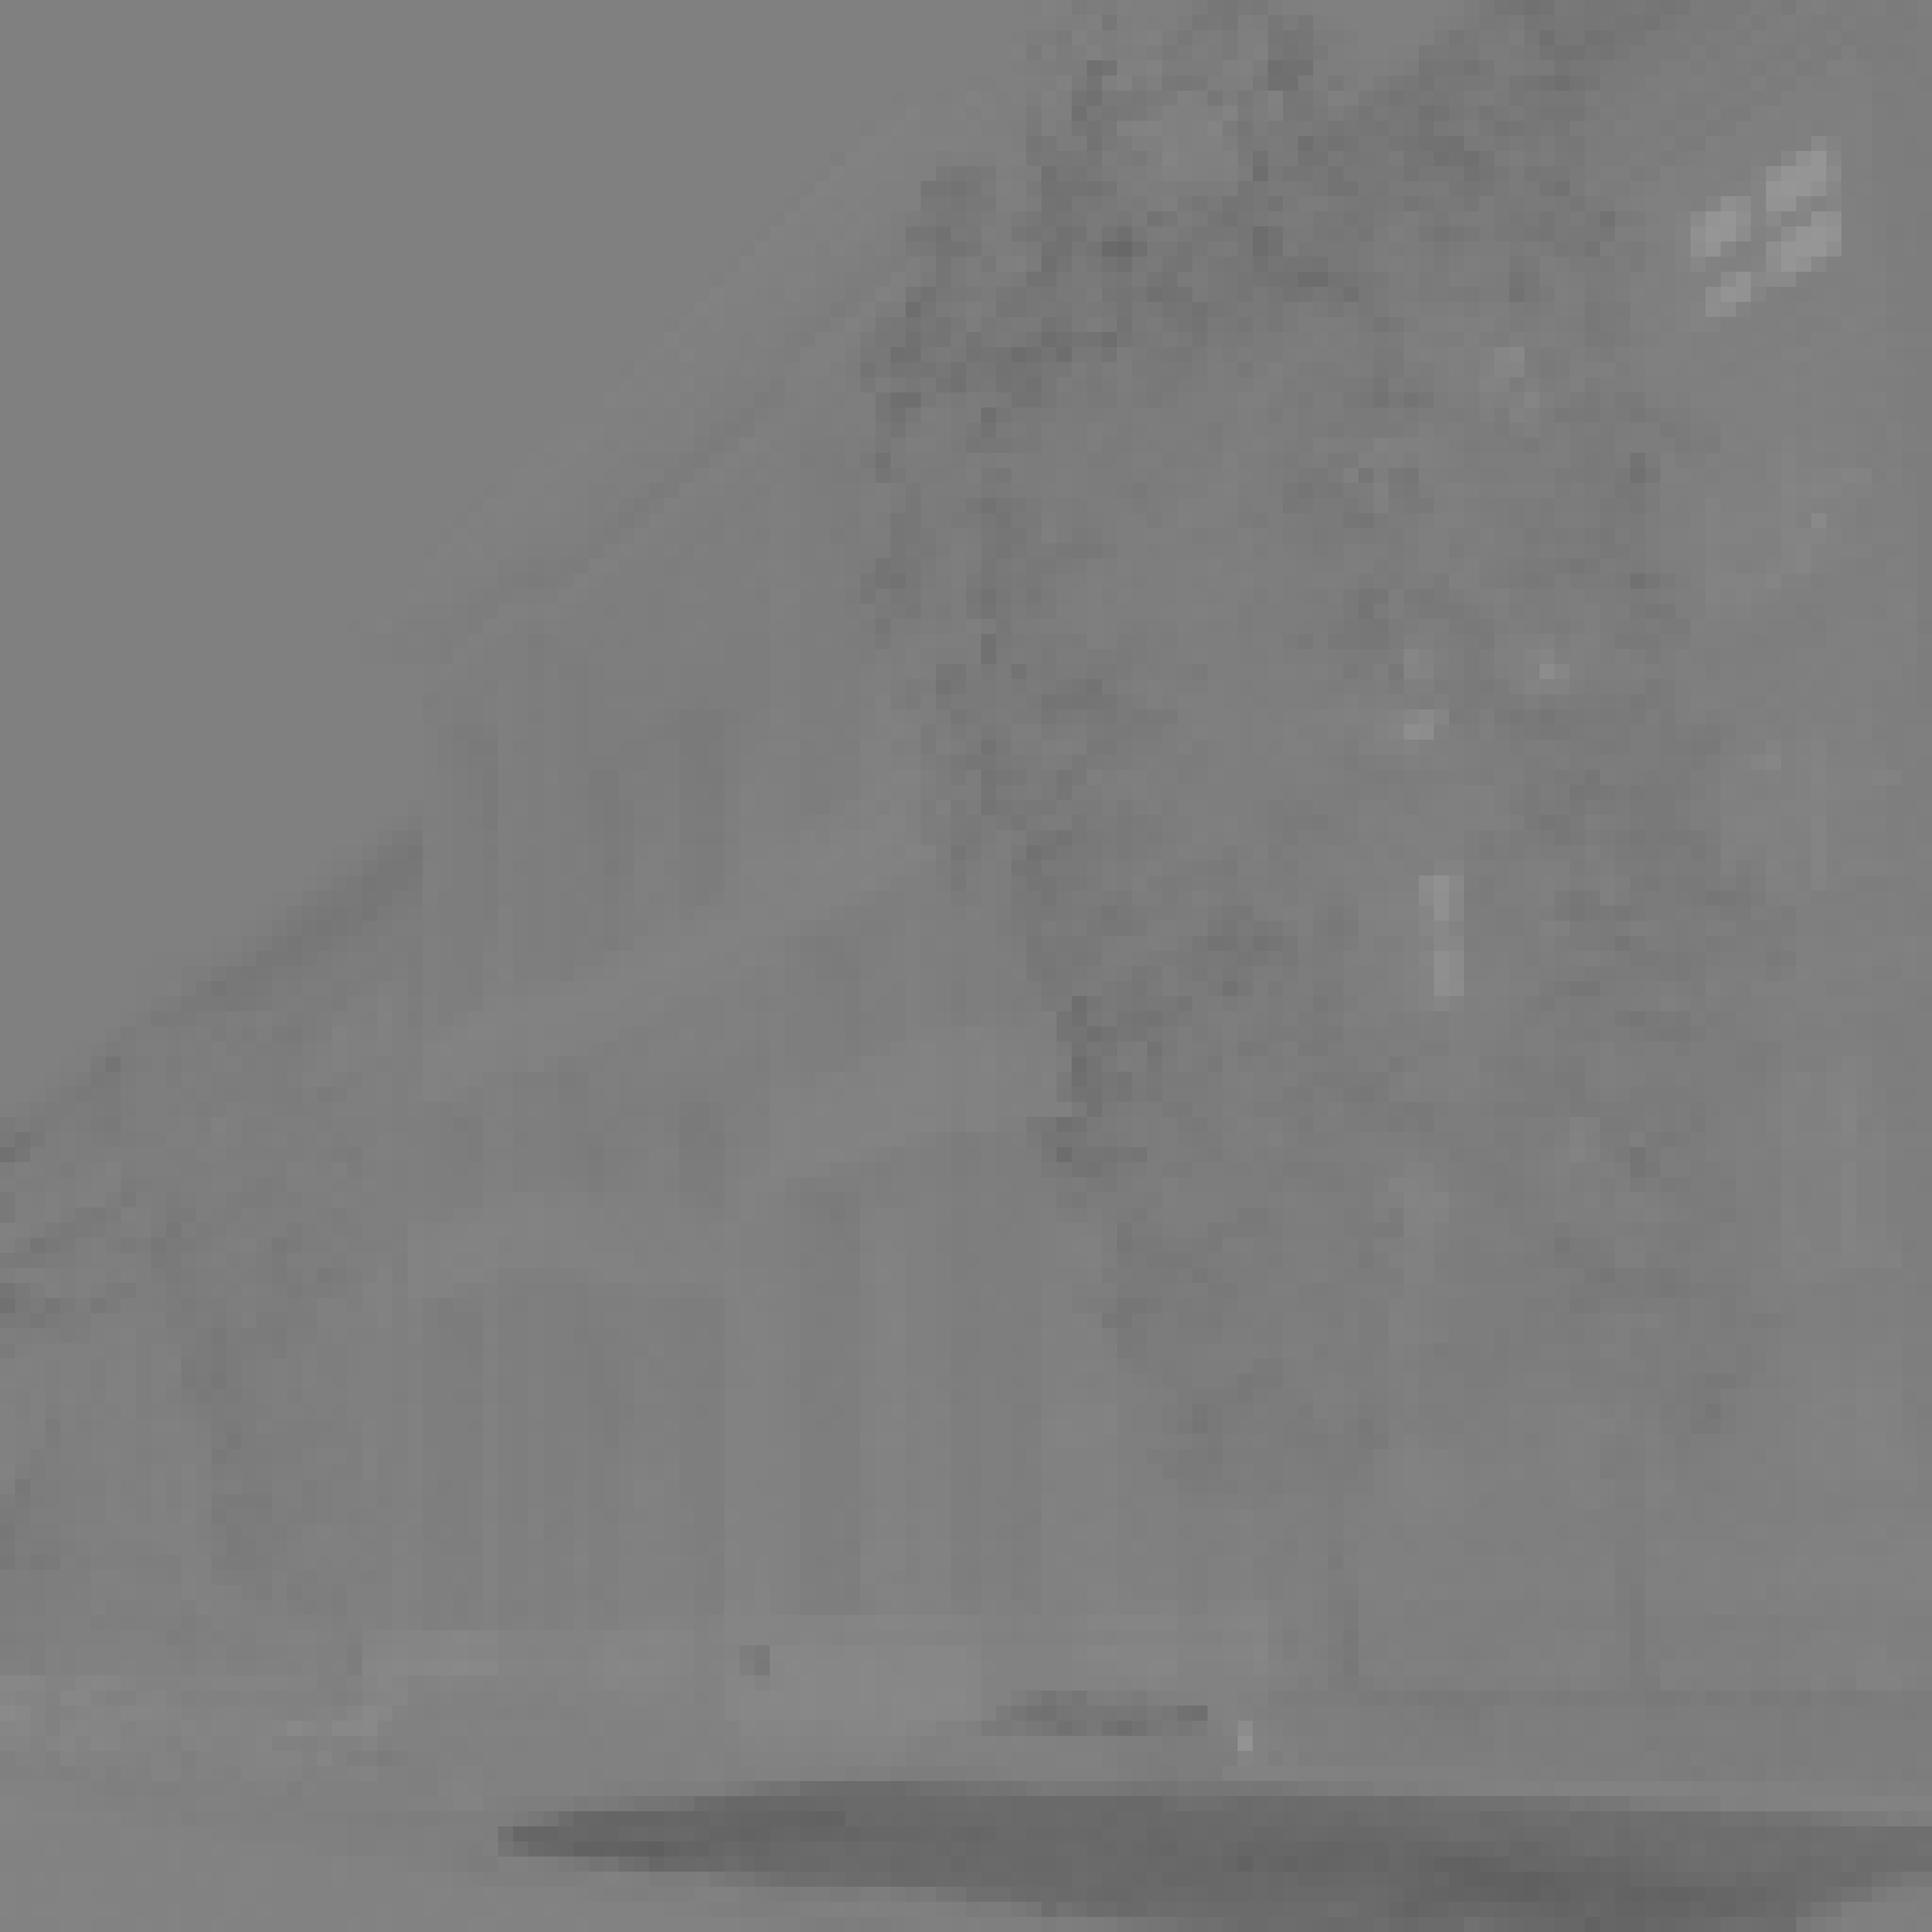
\includegraphics[height=0.25\textwidth]{images/mimuw-square-128-ycbcr-blueness-upscaled.png}};
			\node (redness) at (7,0) {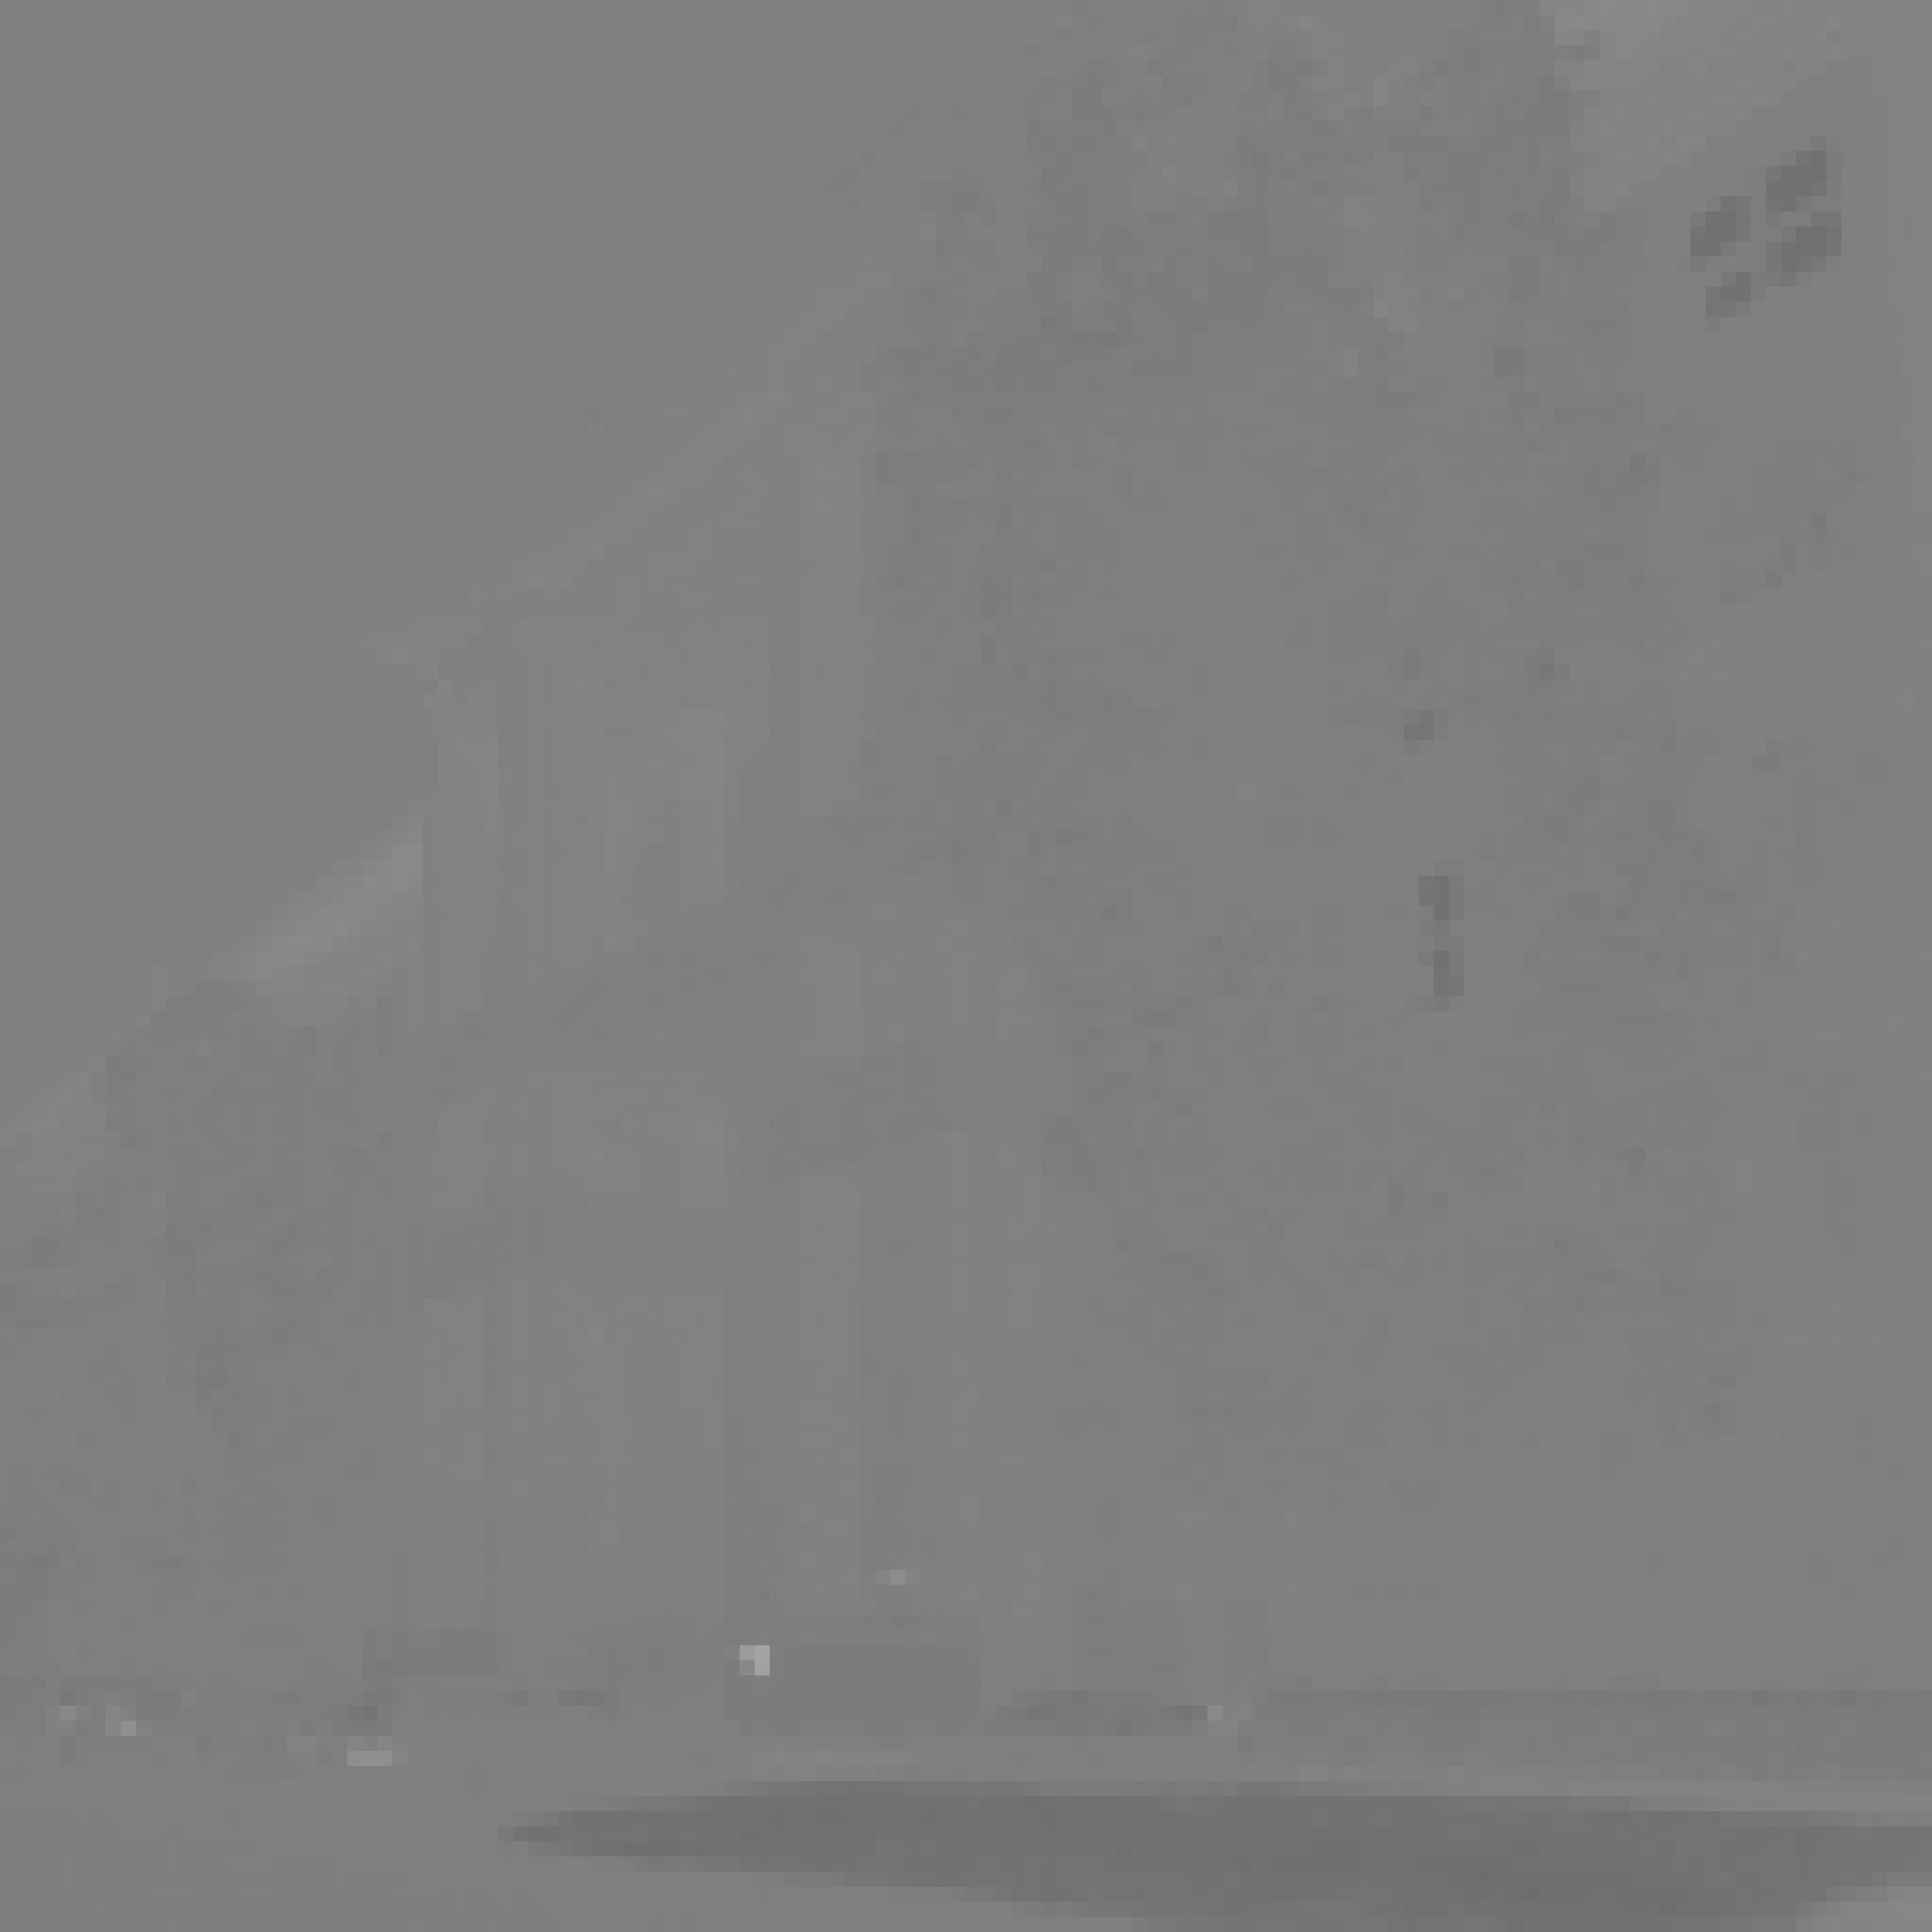
\includegraphics[height=0.25\textwidth]{images/mimuw-square-128-ycbcr-redness-upscaled.png}};
			
			\node[below] at (luma.south) {\textsc{\small Luma}};
			\node[below] at (blueness.south) {\textsc{\small Blueness}};
			\node[below] at (redness.south) {\textsc{\small Redness}};
			
			\draw [<-, shorten >=3pt, shorten <=3pt] (luma) -- (ycbcr);
			\draw [<-, shorten >=3pt, shorten <=3pt] (blueness) -- (ycbcr);
			\draw [<-, shorten >=3pt, shorten <=3pt] (redness) -- (ycbcr);
		\end{tikzpicture}
		\caption{Test image decomposed into YCbCr channels.}
	\end{figure}
\end{frame}

\begin{frame}[c,plain]
	\begin{figure}
		\centering
		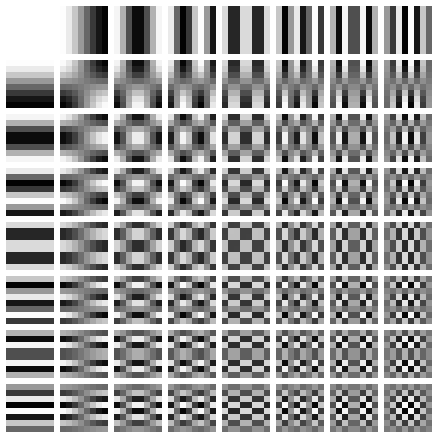
\includegraphics[height=0.6\textwidth]{images/dct-basis.png}
		\caption{Basis for DCT.}
	\end{figure}
\end{frame}

\begin{frame}[c]{Quantization}
\vspace{5pt}
\begin{figure}
	\centering
	\def\QTzero{{16,11,12,14,12,10,16,14,13,14,18,17,16,19,24,40,26,24,22,22,24,49,35,37,29,40,58,51,61,60,57,51,56,55,64,72,92,78,64,68,87,69,55,56,80,109,81,87,95,98,103,104,103,62,77,113,121,112,100,120,92,101,103,99}}
	\begin{tikzpicture}
		\path[fill=white,fill on=<1>] (0,0) rectangle (6.4,6.4);
		\foreach \x[
			evaluate=\x as \startx using {\x*.8}] in {0,...,7}{
			\foreach \y[
				evaluate=\y as \i using int(\y*8+\x),
				evaluate=\y as \value using {\QTzero[\i]},
				evaluate=\y as \starty using {-\y*.8 + 6.4},
				evaluate=\y as \strength using {100*\value/128},
				evaluate=\y as \textcolor using \strength<50?100:0] in {0,...,7}{
				\path[fill=black!\strength!white,fill on=<2->] ($(\startx, \starty)$) rectangle ($(\startx, \starty) + .8*(1,-1) $);
				\node[text=black!\textcolor!white,text on=<2->] at ($(\startx, \starty) + (0.4,-0.4) $) {\value};
			}
		}
		\draw [draw=black!40!white, xstep=.8, ystep=.8] (0,0) grid (6.4,6.4) rectangle (0,0);
	\end{tikzpicture}
	\caption{Sample quantization table for luma component.}
\end{figure}
\end{frame}

\begin{frame}{References}
  \nocite{sayood2017introduction}
  \bibliography{refs}
  \bibliographystyle{abbrv}
\end{frame}

\end{document}